% Options for packages loaded elsewhere
\PassOptionsToPackage{unicode}{hyperref}
\PassOptionsToPackage{hyphens}{url}
\PassOptionsToPackage{dvipsnames,svgnames*,x11names*}{xcolor}
%
\documentclass[
  a4paper, 11pt]{article}
\usepackage{lmodern}
\usepackage{amssymb,amsmath}
\usepackage{ifxetex,ifluatex}
\ifnum 0\ifxetex 1\fi\ifluatex 1\fi=0 % if pdftex
  \usepackage[T1]{fontenc}
  \usepackage[utf8]{inputenc}
  \usepackage{textcomp} % provide euro and other symbols
\else % if luatex or xetex
  \usepackage{unicode-math}
  \defaultfontfeatures{Scale=MatchLowercase}
  \defaultfontfeatures[\rmfamily]{Ligatures=TeX,Scale=1}
\fi
% Use upquote if available, for straight quotes in verbatim environments
\IfFileExists{upquote.sty}{\usepackage{upquote}}{}
\IfFileExists{microtype.sty}{% use microtype if available
  \usepackage[]{microtype}
  \UseMicrotypeSet[protrusion]{basicmath} % disable protrusion for tt fonts
}{}
\makeatletter
\@ifundefined{KOMAClassName}{% if non-KOMA class
  \IfFileExists{parskip.sty}{%
    \usepackage{parskip}
  }{% else
    \setlength{\parindent}{0pt}
    \setlength{\parskip}{6pt plus 2pt minus 1pt}}
}{% if KOMA class
  \KOMAoptions{parskip=half}}
\makeatother
\usepackage{xcolor}
\IfFileExists{xurl.sty}{\usepackage{xurl}}{} % add URL line breaks if available
\IfFileExists{bookmark.sty}{\usepackage{bookmark}}{\usepackage{hyperref}}
\hypersetup{
  pdftitle={Modelos mistos na Engenharia de Avaliações},
  pdfauthor={Luiz F. P. Droubi; Carlos Augusto Zilli; Norberto Hoccheim},
  colorlinks=true,
  linkcolor=red,
  filecolor=Maroon,
  citecolor=green,
  urlcolor=magenta,
  pdfcreator={LaTeX via pandoc}}
\urlstyle{same} % disable monospaced font for URLs
\usepackage[left=2.5cm,right=2.5cm,top=3cm,bottom=2.5cm]{geometry}
\usepackage{longtable,booktabs}
% Correct order of tables after \paragraph or \subparagraph
\usepackage{etoolbox}
\makeatletter
\patchcmd\longtable{\par}{\if@noskipsec\mbox{}\fi\par}{}{}
\makeatother
% Allow footnotes in longtable head/foot
\IfFileExists{footnotehyper.sty}{\usepackage{footnotehyper}}{\usepackage{footnote}}
\makesavenoteenv{longtable}
\usepackage{graphicx,grffile}
\makeatletter
\def\maxwidth{\ifdim\Gin@nat@width>\linewidth\linewidth\else\Gin@nat@width\fi}
\def\maxheight{\ifdim\Gin@nat@height>\textheight\textheight\else\Gin@nat@height\fi}
\makeatother
% Scale images if necessary, so that they will not overflow the page
% margins by default, and it is still possible to overwrite the defaults
% using explicit options in \includegraphics[width, height, ...]{}
\setkeys{Gin}{width=\maxwidth,height=\maxheight,keepaspectratio}
% Set default figure placement to htbp
\makeatletter
\def\fps@figure{htbp}
\makeatother
\setlength{\emergencystretch}{3em} % prevent overfull lines
\providecommand{\tightlist}{%
  \setlength{\itemsep}{0pt}\setlength{\parskip}{0pt}}
\setcounter{secnumdepth}{5}
\usepackage[brazil]{babel}
\usepackage{amsmath}
\usepackage{graphicx}
\usepackage{float}
\usepackage{subfig}
\usepackage{caption}
\usepackage{lastpage}
\usepackage{rotating}
\usepackage{mathrsfs}
\usepackage{bm}
\usepackage{dcolumn}
\setlength{\parindent}{1.25cm} % Default is 15pt.
\usepackage{indentfirst}
% \usepackage{helvet}
% \renewcommand{\familydefault}{\sfdefault}
% \usepackage{newtxtext,newtxmath} % mais nova para Times.
%\usepackage{mathptmx} % para Times New Roman (preferível newtxtext)
% \usepackage{Times} % para Times New Roman (obsoleto)
\usepackage{fontspec} % para Arial e/ou Times (xelatex ou luatex)
\setmainfont{Arial}
\newcommand{\pkg}[1]{{\normalfont\fontseries{b}\selectfont #1}}
\let\proglang=\textsf
\let\code=\texttt
\usepackage{fancyhdr}
% Turn on the style
\pagestyle{fancy}
% Clear the header and footer
\fancyhead{}
\fancyfoot{}
% Set the right side of the footer to be the page number
\fancyfoot[R]{\thepage~/~\pageref{LastPage}}
\usepackage{booktabs}
\usepackage{longtable}
\usepackage{array}
\usepackage{multirow}
\usepackage{wrapfig}
\usepackage{float}
\usepackage{colortbl}
\usepackage{pdflscape}
\usepackage{tabu}
\usepackage{threeparttable}
\usepackage{threeparttablex}
\usepackage[normalem]{ulem}
\usepackage{makecell}

\title{Modelos mistos na Engenharia de Avaliações}
\usepackage{etoolbox}
\makeatletter
\providecommand{\subtitle}[1]{% add subtitle to \maketitle
  \apptocmd{\@title}{\par {\large #1 \par}}{}{}
}
\makeatother
\subtitle{Possibilidades e aplicações}
\author{Luiz F. P. Droubi\footnote{SPU/SC,
  \href{mailto:lfpdroubi@gmail.com}{\nolinkurl{lfpdroubi@gmail.com}}} \and Carlos Augusto Zilli\footnote{IFSC,
  \href{mailto:carlos.zilli@ifsc.edu.br}{\nolinkurl{carlos.zilli@ifsc.edu.br}}} \and Norberto Hoccheim\footnote{UFSC,
  \href{mailto:hochheim@gmail.com}{\nolinkurl{hochheim@gmail.com}}}}
\date{14/10/2020}

\begin{document}
\maketitle

\hypertarget{introduuxe7uxe3o}{%
\section{Introdução}\label{introduuxe7uxe3o}}

Na Engenharia de Avaliações, assim como em diversos ramos das ciências
sociais, a abordagem padrão para lidar com a heteregoneidade amostral é
a modelagem com efeitos fixos. Este tipo de abordagem permite a
segregação dos dados da amostra em diferentes agrupamentos, através da
utilização de variáveis \emph{dummies}\footnote{Ou variáveis dicotômicas
  em grupo. Neste trabalho estas variáveis serão tratadas simplesmente
  pelo termo em inglês \emph{dummies}.} que indicam a que agrupamento
pertence cada dado amostral.

Como será visto, no entanto, este tipo de modelagem elimina a
possibilidade de \emph{explicar} a variância \emph{entre} os diversos
grupos de dados. Na Engenharia de Avaliações, quando o objetivo é a
previsão de valores de um imóvel em específico, isto não acarreta em
nenhum problema, a não ser que existam poucos dados nos agrupamentos, o
que acaba por prejudicar a estimação.

No entanto, quando o objetivo é a explicação do mercado, a modelagem por
efeitos fixos deixa a desejar: o máximo que se pode obter de um modelo
de efeitos fixos é a magnitude do efeito da localização em um
determinado agrupamento.\footnote{Plümper e Troeger (2007) propuseram
  efetuar a decomposição vetorial do modelo de efeitos fixos para a
  modelagem de níveis mais altos, porém este método foi fortemente
  criticado por sua imprecisão no cálculo dos erros-padrão e ainda
  possui as desvantagens de não ser possível a estimação de níveis
  superiores a 2 e de requerer a estimação em diferentes estágios (BELL;
  JONES, \protect\hyperlink{ref-bell2015}{2015}, pp. 140--141).} Nada
que possa explicar o contexto pode ser incluído na análise, já que toda
a variância no nível dos agrupamentos é absorvida pelas \emph{dummies}.

Nos modelos mistos, além dos efeitos fixos ligados à explicação do valor
dos imóveis, tais como área, número de quartos e/ou banheiros, e outros,
efeitos aleatórios são utilizados para lidar com a heterogeneidade da
amostra, seja devido ao contexto, seja devido ao tempo, já que os
modelos mistos possuem grande aplicação na modelagem de dados em painel
ou séries temporais.

O objetivo deste trabalho é a apresentação dos modelos mistos e suas
possibilidades de aplicação na Engenharia de Avaliações. No caso da
modelagem de dados em seção transversal (corte), será mostrado como os
modelos mistos podem ser úteis na elaboração de plantas de valores
genéricos. Além disto, será discutido brevemente a aplicação dos modelos
mistos para dados em painel, o que pode ser útil, na Engenharia de
Avaliaçãoes, na construção de índices de preços de imóveis.

\hypertarget{revisuxe3o-bibliogruxe1fica}{%
\section{Revisão Bibliográfica}\label{revisuxe3o-bibliogruxe1fica}}

Os modelos de efeitos fixos são uma espécie de ``padrão ouro'' em
diversos ramos da ciência para lidar com a heterogeneidade amostral. No
entanto, de acordo com Bell \emph{et al.}
(\protect\hyperlink{ref-bell2019}{2019}, p. 1052), os modelos mistos bem
especificados oferecem uma abordagem muito mais completa destes tipos de
dados do que a modelagem por efeitos fixos.

Segundo Bell \emph{et al.} (\protect\hyperlink{ref-bell2019}{2019}, p.
1051), existe uma confusão na literatura a respeito dos modelos mistos,
no que tange à aglutinação em uma modelagem de diversos tipos de
efeitos, fixos e aleatórios, sendo que os modelos mistos mais complexos
tem sido chamados, erroneamente, de modelos híbridos.

Os modelos mistos também podem ser confundidos com modelos multiníveis
ou hierárquicos, uma vez que estes últimos são um caso particular dos
primeiros, \emph{i.e} os modelos hierárquicos são modelos mistos em que
os dados se apresentam de maneira aninhada (imóveis se agrupam em
bairros, que por sua vez se agrupam em regiões e assim por diante), o
que possibilita a sua modelagem de maneira hierárquica. No entanto, se
os dados se agrupam em diferentes grupamentos independentes, não
aninhados, a modelagem hierárquica não se aplica, porém estes tipos de
dados podem também ser modelados pelos modelos mistos. Em suma, todo
modelo misto é um modelo hierárquico, mas o inverso não se aplica (BATES
et al., \protect\hyperlink{ref-Bates}{2015}).

\hypertarget{modelagem-por-efeitos-fixos}{%
\subsection{Modelagem por efeitos
fixos}\label{modelagem-por-efeitos-fixos}}

A modelagem por efeitos fixos é frequentemente aplicada na Engenharia de
Avaliações, assim como em diversas outras áreas da ciência (BELL et al.,
\protect\hyperlink{ref-bell2019}{2019}, p. 1057), apesar desta
terminologia não ser sempre empregada.

Um modelo de efeitos fixos nada mais é do que um modelo em que a
heterogeneidade da amostra é ``saneada'' através da inclusão de
variáveis \emph{dummies} representando cada agrupamento de dados. Após a
inclusão destas variáveis saneando a amostra, a estimação é feita pelo
métodos dos mínimos quadrados ordinários.

A modelagem por efeitos fixos pode ser escrita conforme a equação
\ref{eq:fixef}, onde a variância entre os agrupamentos de dados
(variância de nível mais alto) é modelada através de variáveis
\emph{dummies} \(D_j\) (BELL; JONES,
\protect\hyperlink{ref-bell2015}{2015}, p. 138):

\begin{equation} \label{eq:fixef}
y_{ij} = \sum_{j=1}^{j}\beta_{0j}D_j + \beta_1 x_{ij} + \varepsilon_{ij}
\end{equation}

No entanto, uma outra maneira mais conveniente de escrever a formulação
de efeitos fixos, para a comparação que se pretende, equivalente à
primeira, pode ser vista na equação \ref{eq:fixef2} (BELL et al.,
\protect\hyperlink{ref-bell2019}{2019}, p. 1058):

\begin{equation} \label{eq:fixef2}
y_{ij} = \beta_1 (x_{ij} - \bar{x}_j) + (\upsilon_j + \varepsilon_{ij}) 
\end{equation}

Onde \(\upsilon_j\) é um termo discreto para cada agrupamento de
dados\footnote{O termo \(\upsilon_j\) é o intercepto de cada
  agrupamento, quando se ajusta um modelo sem intercepto.}. Os índices
\(i\) e \(j\) se referem aos dois níveis de análise: \(i\), neste caso,
representa o nível dos indivíduos e \(j\) o nível dos agrupamentos.
\(\varepsilon_{ij}\) é um termo de erro aleatório com distribuição
supostamente normal, média zero e desvio-padrão
\(\sigma_{\varepsilon}^2\).

Na prática, no entanto, a formulação acima raramente é utilizada, pois
perde-se um grau de liberdade na estimação de um intercepto para cada
bairro, quando se pode utilizar um nível de referência e estimar apenas
a diferença entre os níveis de cada agrupamento em relação a este nível
de referência, como ilustrado na equação \ref{eq:fixef3} (BELL et al.,
\protect\hyperlink{ref-bell2019}{2019}, p. 1058):

\begin{equation} \label{eq:fixef3}
(y_{ij} - \bar{y}_i) = \beta_1 (x_{ij} - \bar{x}_j) + (\varepsilon_{ij}) 
\end{equation}

\hypertarget{modelagem-por-efeitos-mistos}{%
\subsection{Modelagem por efeitos
mistos}\label{modelagem-por-efeitos-mistos}}

Existem diversas formas de se utilizar os modelos mistos. Neste trabalho
apresentam-se diversas possibilidades, desde a abordagem mais simples,
que possibilita uma melhor comparação com o modelo de efeitos fixos,
muito conhecido na Engenharia de Avaliações, até a abordagem mais
complexa, a formulação REWB (Random Effects Within-Between).

\hypertarget{modelo-de-efeitos-mistos-simples}{%
\subsubsection{Modelo de efeitos mistos
simples}\label{modelo-de-efeitos-mistos-simples}}

A modelagem por efeitos mistos considera, além dos efeitos fixos, um
termo de efeitos aleatórios (BELL et al.,
\protect\hyperlink{ref-bell2019}{2019}, p. 1059). Uma das maneiras de
escrever a formulação de efeitos mistos pode ser vista na equação
\ref{eq:mixef}.

\begin{equation} \label{eq:mixef}
y_{ij} = \beta_0 + \beta_1^{RE} x_{ij} + \beta_2 z_j + (\upsilon_j + \varepsilon_{ij}) 
\end{equation}

No caso da equação \ref{eq:mixef}, o termo \(\upsilon_j\) é um termo
estocástico de efeitos aleatórios para os indivíduos, suposto
normalmente distribuído e com média zero, ou seja
\(\upsilon_j \sim N(0, \sigma_{\upsilon}^2)\) (BELL et al.,
\protect\hyperlink{ref-bell2019}{2019}, p. 1055). A variável \(x_{ij}\)
é uma variável de nível 1, variante entre os indivíduos e a variável
\(z_j\) é uma variável de nível 2, invariante entre os agrupamentos,
\emph{i.e.} a variável \(z_j\) não é uma variável hedônica dos imóveis,
mas uma variável que representa todo um grupo de imóveis.\footnote{É
  possível utilizar os models mistos sem a utilização de qualquer
  variável de segundo nível, obtendo-se um modelo de interceptos
  aleatórios.}

Neste tipo de modelagem estimam-se, além dos coeficientes das variáveis
de nível mais baixo, \(\beta_0\) e \(\beta_1\), o(s) coeficiente(s)
da(s) variável(eis) de segundo nível \(\beta_2\) e os parâmetros
\(\sigma_\upsilon^2\) e \(\sigma_\varepsilon^2\), ou seja, as variâncias
de primeiro e segundo nível, respectivamente.

A diferença de nível entre as variáveis pode ser melhor compreendida ao
se dividir a modelagem em dois níveis (modelagem hierárquica), como pode
ser visto nas equações \ref{eq:micro} e \ref{eq:macro}:

\begin{equation} \label{eq:micro}
y_{ij} = \beta_{0j} + \beta_1^{RE} x_{ij} + \varepsilon_{ij} 
\end{equation}

\begin{equation} \label{eq:macro}
\beta_{0j} = \beta_0 + \beta_2 z_{j} + \upsilon_{j} 
\end{equation}

Segundo Bell e Jones (\protect\hyperlink{ref-bell2015}{2015}, pp.
135--136), a equação \ref{eq:micro} é chamada de parte micro, enquanto a
equação \ref{eq:macro} é chamada de parte macro da formulação de efeitos
mistos, que são estimadas em conjunto ao substituir \ref{eq:macro} em
\ref{eq:micro} para se obter o modelo misto da equação \ref{eq:mixef}.

Em suma, para Bell \emph{et al.}
(\protect\hyperlink{ref-bell2019}{2019}, p. 1061), a grande diferença
entre a formulação de efeitos fixos e a formulação de efeitos mistos
está na maneira como as modelagens tratam os agrupamentos de dados, se
de maneira discreta (efeitos fixos) ou de maneira aleatória (efeitos
aleatórios). Enquanto na modelagem de efeitos fixos são adicionadas
variáveis \emph{dummies} discretas para a modelagem dos diferentes
agrupamentos, na modelagem de efeitos aleatórios é considerado que a
diferença entre os dados de diferentes agrupamentos pode ser modelada
por uma variável aleatória normal.

Enquanto nos modelos mistos a variância é dividida em duas partes, uma
ao nível dos indivíduos e outra ao nível dos agrupamentos, nos modelos
de efeitos fixos a variância entre os agrupamentos é totalmente
absorvida pelas variáveis \emph{dummies}, que consomem todos os graus de
liberdade do segundo nível hierárquico, eliminando dessa forma qualquer
possibilidade de introdução de variáveis como \(z_j\), na equação
\ref{eq:mixef} (BELL; JONES, \protect\hyperlink{ref-bell2015}{2015}, p.
139).

Segundo os autores citados, ainda, esta visão não é unânime: na
econometria, por exemplo, é considerado que a diferença fundamental
entre as modelagens de efeitos fixos e efeitos mistos está de fato na
hipótese considerada pelos modelos mistos de que não há correlação dos
efeitos aleatórios (representados por \(\upsilon_i\)) e os regressores
(\(x_ij\)), o que é permitido na modelagem de efeitos fixos (BELL et
al., \protect\hyperlink{ref-bell2019}{2019}, p. 1060).

Deve-se notar ainda que os modelos mistos, tal como apresentados na
equação \ref{eq:mixef}, ainda podem ser facilmente estendidos para
incorporar outros níveis hierárquicos mais altos, ou ainda a
variabilidade não apenas para os interceptos, mas também para os
coeficientes das variáveis explicativas, com o consumo de apenas mais um
grau de liberdade, como pode ser visto na equação \ref{eq:mixef2}, onde
além do termo aleatório relacionado aos interceptos é adicionado outro
termo aleatório, \(\gamma_j \sim N(0, \sigma^2_\gamma)\), relacionado às
inclinações, formando assim um modelo de interceptos e inclinações
aleatórias (BELL et al., \protect\hyperlink{ref-bell2019}{2019}, p.
1052):

\begin{equation} \label{eq:mixef2}
y_{ij} = (\beta_0 + \upsilon_j) + (\beta_1 + \gamma_j) x_{ij} + \beta_2 z_j + \varepsilon_{ij}
\end{equation}

Na modelagem por efeitos fixos seriam necessárias a inclusão de diversos
termos de interação para a modelagem de uma inclinação diferente para
cada agrupamento, gerando um modelo cuja estimação é extremamente
custosa em termos de graus de liberdade.

\hypertarget{formulauxe7uxe3o-de-mundlak}{%
\subsubsection{Formulação de
Mundlak}\label{formulauxe7uxe3o-de-mundlak}}

Esta formulação consiste da introdução de um termo adicional à parte
macro do modelo, que leva em conta a variação \emph{entre} os grupos
(\emph{between effect}), de maneira que a equação \ref{eq:macro}
torna-se:

\begin{equation} \label{eq:macro2}
\beta_{0j} = \beta_0 + \beta_2 z_{j} + \beta_3 \bar{x}_j + \upsilon_{j} 
\end{equation}

A combinação das equações \ref{eq:micro} e \ref{eq:macro2} toma a forma
da equação \ref{eq:mundlak}, que é conhecida na literatura como
formulação de Mundlak (BELL; JONES,
\protect\hyperlink{ref-bell2015}{2015}, p. 1055):

\begin{equation} \label{eq:mundlak}
y_{ij} = \beta_0 + \beta_{1} x_{ij} + \beta_{3}\bar{x}_j+ \beta_2 z_j + (\upsilon_j + \varepsilon_{ij}) 
\end{equation}

Segundo Bell \emph{et al.} (\protect\hyperlink{ref-bell2019}{2019}, p.
1055), na formulação de Mundlak o efeito contextual, representado na
equação \ref{eq:mundlak} pelo termo \(\beta_{3}\) (algumas vezes escrito
como \(\beta_{C}\)), é de interesse, pois mostra a \emph{diferença}
entre os efeitos \emph{dentro} (\emph{within effect}) e \emph{entre}
(\emph{between effect}) os grupos.

Na prática, os modelos de Mundlak e os modelos de efeitos fixos
estimarão exatamente os mesmos valores para os coeficientes de efeitos
dentro dos agrupamentos (\emph{within effects}), representado na
formulação acima pelo termo \(\beta_1\), algumas vezes escrito
\(\beta_{W}\) (BELL et al., \protect\hyperlink{ref-bell2019}{2019}, p.
1057).

Esta formulação, segundo Bell \emph{et al.}
(\protect\hyperlink{ref-bell2019}{2019}, p. 1056), é particularmente
interessante para a análise de dados em seção transversal, pois o
coeficiente \(\beta_C\) representa o efeito da mundança de grupo de um
indivíduo, mantidas as suas características.

Na Engenharia de Avaliações, por exemplo, o valor de \(\beta_C\) pode
representar qual é a influência de uma característica no valor de um
lote-padrão, quando este lote-padrão muda de um bairro ou zona para
outro, o que é particularmente interessante para a confecção de planta
de valores genéricos. Por exemplo, imagine-se que se esteja tratando da
variável área do lote: enquanto \(\beta_W\) representa o efeito da
mudança de área de um imóvel dentro dos agrupamentos, \(\beta_C\)
representará o efeito da mudança da área média do agrupamento sobre o
valor do lote, ou seja, qual o efeito do contexto sobre o valor do lote.

\hypertarget{formulauxe7uxe3o-within-between}{%
\subsubsection{Formulação
Within-Between}\label{formulauxe7uxe3o-within-between}}

Uma maneira às vezes mais adequada de escrever a formulação de modelos
mistos consiste na separação total dos efeitos dentro dos agrupamentos
dos efeitos entre os agrupamentos, o que é conhecido na literatura por
formulação \emph{within-between}. Esta formulação é a mais genérica,
capaz de modelar diversos efeitos separadamente e é particularmente
interessante na análise de dados em painéis ou séries temporais, dada a
sua melhor interpretabilidade para estes tipos de dados (BELL; JONES,
\protect\hyperlink{ref-bell2015}{2015}, p. 143).

Partindo da formulação de Mundlak, os efeitos \emph{within} e
\emph{between} podem ter seus efeitos totalmente separados pela divisão
do coeficiente \(\beta_3\) da equação \ref{eq:mundlak}, escrevendo-o
explicitamente como uma diferença em relação ao coeficiente \(\beta_1\),
conforme mostrado pela equação \ref{eq:rewb1}

\begin{equation} \label{eq:rewb1}
y_{ij} = \beta_0 + \beta_1 x_{ij} + (\beta_{4} - \beta_1) \bar{x}_j+ \beta_2 z_j + (\upsilon_j + \varepsilon_{it}) 
\end{equation}

Rearranjando conveniente a equação \ref{eq:rewb1}, chega-se à formulação
REWB, como mostra a equação \ref{eq:rewb2}:

\begin{equation} \label{eq:rewb1}
y_{ij} = \beta_0 + \beta_1 (x_{ij} - \bar{x}_j) + \beta_4 \bar{x}_j+ \beta_2 z_j + (\upsilon_j + \varepsilon_{it}) 
\end{equation}

Mais uma vez é possível, ainda, a adição de inclinações aleatórias nesta
formulação, obtendo-se assim a formulação mais genérica possíve, como
pode ser visto na equação \ref{eq:rewb2}:

\begin{equation} \label{eq:rewb2}
y_{ij} = \mu + \beta_{W} (x_{ij} - \bar{x}_j) + \beta_{B}\bar{x}_j+ 
\beta_2 z_j + \upsilon_{j0} + \upsilon_{j1} (x_{ij} - \bar{x}_j) + \varepsilon_{ij0} 
\end{equation}

Onde o termo \(\upsilon_{j0}\) está relacionado à aleatoriedade do
intercepto e o termo \(\upsilon_{j1}\) está relacionado à aleatoriedade
do coeficiente da variável \(x\).

\hypertarget{considerauxe7uxf5es-sobre-a-pertinuxeancia-de-cada-modelagem}{%
\subsection{Considerações sobre a pertinência de cada
modelagem}\label{considerauxe7uxf5es-sobre-a-pertinuxeancia-de-cada-modelagem}}

Segundo Bell e Jones (\protect\hyperlink{ref-bell2015}{2015}, p. 143),
um modelo de efeitos fixos pode ser visto como uma forma de modelo de
efeitos mistos onde a variância nos níveis mais altos é restringida a
infinito. Desta maneira, para Bell e Jones
(\protect\hyperlink{ref-bell2015}{2015}), os modelos de efeitos mistos
são muito mais interessantes do que os modelos de efeitos fixos, já que
além de propiciarem todas as informações que os modelos de efeitos fixos
propiciam, eles ainda tem possibilidade de ir além e fornecer outras
informações que os modelos de efeitos fixos não fornecem, como a
separação dos efeitos de uma variável \emph{entre} os agrupamentos e
\emph{dentro} dos agrupramentos. Para Bell \emph{et al.}
(\protect\hyperlink{ref-bell2019}{2019}, p. 1060), para o efeito
\emph{dentro} dos agrupamentos, os resultados estimados pela formulação
REWB ou pela formulação de Mundlak serão rigorosamente os mesmos obtidos
pelo modelo de efeitos fixos. No entanto, enquanto os modelos de REWB e
de Munlak fornecem informações a respeito dos efeitos \emph{entre} os
agrupamentos, os modelos de efeitos fixos não são capazes de fornecer
qualquer informação a este respeito, já que a variância de nível mais
alto foi restringida.

Deve ser feita uma distinção também entre os objetivos da modelagem: na
Engenharia de Avaliações, se o objetivo for determinar o valor de um
imóvel em específico a partir de uma amostra heterogênea, sem a
pretensão de explicar a diferença de valores entre os diversos
agrupamentos, a formulação de efeitos fixos é suficiente, exceto no caso
de não haver dados suficientes para uma boa estimação dentro de cada
agrupamento. Já quando o objetivo é a obtenção do valor de um imóvel
padrão em diferentes agrupamentos, como na elaboração de uma PVG, a
modelagem por efeitos mistos é a mais adequada, especialmente se não se
dispõe de dados disponíveis para os diferentes agrupamentos, mas apenas
para uma parte (representativa) deles, caso em que a adição de variáveis
de nível mais alto podem ser utilizadas para a previsão de valores nos
agrupamentos não-amostrados.

Deve ser observado também que a hipótese de modelar os diversos
agrupamentos como uma variável aleatória é razoável apenas quando o
número de agrupamentos for grande o suficiente. Para poucos
agrupamentos, a modelagem por efeitos fixos ainda parece ser mais
adequada (ver BELL et al., \protect\hyperlink{ref-bell2019}{2019}, p.
1071).

Também deve ser observado, ainda, que a utilização da formulação simples
para modelos mistos, como a da equação \ref{eq:mixef}, como muitas vezes
se encontra na prática (ver CICHULSKA; CELLMER,
\protect\hyperlink{ref-polonia}{2018}), não é tão interessante como a
aplicação das modelagens REWB e de Mundlak. No entanto, a aplicação da
formulação REWB e de Mundlak só faz sentido se houver efetivamente uma
diferença entre os efeitos dentro e entre os agrupamentos. Caso
\(\beta_{1W} = \beta_{2B}\) (REWB) ou \(\beta_{2C} = 0\) (Mundlak), não
faz sentido utilizar estas formulações e a formulação simples de efeitos
mistos (equação \ref{eq:mixef}) deve ser a adotada (BELL et al.,
\protect\hyperlink{ref-bell2019}{2019}, p. 1058).

\hypertarget{estimauxe7uxe3o-em-modelos-mistos}{%
\subsection{Estimação em modelos
mistos}\label{estimauxe7uxe3o-em-modelos-mistos}}

Existem diversas formas de estimação para os modelos mistos. Segundo
Jones e Bullen (\protect\hyperlink{ref-jones1994}{1994}, p. 258), até
meados da década de 80 a falta de algoritmos de estimação gerais
limitava severamente a aplicação da modelagem multinível. Durante a
década de 80, contudo, três algoritmos tornaram-se disponíveis, sendo os
mais importantes o procedimento de Goldstein
(\protect\hyperlink{ref-goldstein}{1986}), que consistia na estimação
dos mínimos quadrados generalizados de maneira iterativa e um algoritmo
denominado Fischer-scoring (LONGFORD,
\protect\hyperlink{ref-longford}{1987}).

Mais recentemente, a estimação através da penalização de mínimos
quadrados ponderados tem se mostrado superior em termos computacioanis
(BATES,
\protect\hyperlink{ref-Bates3}{2018}\protect\hyperlink{ref-Bates3}{a},
\protect\hyperlink{ref-Bates2}{2018}\protect\hyperlink{ref-Bates2}{b}).

Os detalhes da implementação estão além do escopo deste artigo e podem
ser vistos em Bates
(\protect\hyperlink{ref-Bates2}{2018}\protect\hyperlink{ref-Bates2}{b}).

Segundo Clark (\protect\hyperlink{ref-clark2019shrinkage}{2019}), uma
das características mais fortes da estimação em modelos mistos está
relacionada ao encolhimento, ou seja, a suposição da normalidade dos
efeitos aleatórios tem o efeito de penalizar mais as observações mais
discrepantes, fazendo com que os interceptos e coeficientes previstos se
encolham em direção aos valores médios.

Isto é particularmente interessante no caso da presença de agrupamentos
com pequeno número de dados: enquanto nos modelos de efeitos fixos os
valores dos coeficientes e interceptos se superajustam a estes poucos
dados, gerando valores extremos, nos modelos de efeitos mistos, os
agrupamentos com menos dados e valores potencialmente mais extremos, tem
os valores dos coeficientes e interceptos encolhidos em relação à média.
É comum se referir a este efeito como um ``empréstimo de força'',
\emph{i.e.} a previsão nos agrupamentos de menor número de dados é
fortalecida pelo ``empréstimo'' de dados de outros agrupamentos (JONES;
BULLEN, \protect\hyperlink{ref-jones1994}{1994}, p. 260).

\hypertarget{estudo-de-caso}{%
\section{Estudo de Caso}\label{estudo-de-caso}}

Para o estudo de caso foi utilizada a implementação do pacote \pkg{lme4}
(BATES et al., \protect\hyperlink{ref-Bates}{2015}) no \proglang{R},
versão 4.0.2 (R CORE TEAM, \protect\hyperlink{ref-R}{2020}).

\hypertarget{criauxe7uxe3o-de-dados-via-simulauxe7uxe3o}{%
\subsection{Criação de dados via
simulação}\label{criauxe7uxe3o-de-dados-via-simulauxe7uxe3o}}

Foram criados 500 dados de lotes, divididos igualmente em 10 bairros, a
partir de simulação com o auxílio do software \textbf{R}.

Os dados foram criados conforme a equação abaixo \ref{eq:EC1} e
\ref{eq:EC2}, abaixo:

\begin{align}
ValorUnitario &= \beta_{0j} - 3,0 Area + \varepsilon_{ij}  \label{eq:EC1}\\
\beta_{0j} &= \beta_0 + 4000 A_{Vj} + 5 \overline{Area_j} + \upsilon_j \label{eq:EC2}
\end{align}

Onde:

\begin{enumerate}
\def\labelenumi{\arabic{enumi}.}
\tightlist
\item
  \(Area\) são as áreas dos lotes;
\item
  \(A_{Vj}\) é uma variável de nível 2 que representa a porcentagem de
  áreas verdes em cada bairro, em relação à área total;
\item
  \(\overline{Area_j}\) é a área média dos lotes em cada bairro;
\item
  \(\varepsilon_{ij}\) é o termo de erro no primeiro nível de análise;
\item
  \(\upsilon_j\) é o termo de erro no segundo nível de análise.
\end{enumerate}

Os parâmetros adotados para cada variável podem ser vistos na tabela 1:

\begin{longtable}[]{@{}lrcrc@{}}
\caption{Parâmetros utilizados para simulação dos dados.}\tabularnewline
\toprule
\begin{minipage}[b]{0.22\columnwidth}\raggedright
Variável\strut
\end{minipage} & \begin{minipage}[b]{0.10\columnwidth}\raggedleft
Tipo\strut
\end{minipage} & \begin{minipage}[b]{0.10\columnwidth}\centering
Distribuição\strut
\end{minipage} & \begin{minipage}[b]{0.25\columnwidth}\raggedleft
Parâmetros\strut
\end{minipage} & \begin{minipage}[b]{0.19\columnwidth}\centering
Obs.\strut
\end{minipage}\tabularnewline
\midrule
\endfirsthead
\toprule
\begin{minipage}[b]{0.22\columnwidth}\raggedright
Variável\strut
\end{minipage} & \begin{minipage}[b]{0.10\columnwidth}\raggedleft
Tipo\strut
\end{minipage} & \begin{minipage}[b]{0.10\columnwidth}\centering
Distribuição\strut
\end{minipage} & \begin{minipage}[b]{0.25\columnwidth}\raggedleft
Parâmetros\strut
\end{minipage} & \begin{minipage}[b]{0.19\columnwidth}\centering
Obs.\strut
\end{minipage}\tabularnewline
\midrule
\endhead
\begin{minipage}[t]{0.22\columnwidth}\raggedright
Área do lote (\(Area\))\strut
\end{minipage} & \begin{minipage}[t]{0.10\columnwidth}\raggedleft
Quantitativa\strut
\end{minipage} & \begin{minipage}[t]{0.10\columnwidth}\centering
Normal\strut
\end{minipage} & \begin{minipage}[t]{0.25\columnwidth}\raggedleft
\(\mu = 400 \ a \ 500, \sigma = 50\)\strut
\end{minipage} & \begin{minipage}[t]{0.19\columnwidth}\centering
-\strut
\end{minipage}\tabularnewline
\begin{minipage}[t]{0.22\columnwidth}\raggedright
Área média (\(\overline{Area}\))\strut
\end{minipage} & \begin{minipage}[t]{0.10\columnwidth}\raggedleft
Quantitativa\strut
\end{minipage} & \begin{minipage}[t]{0.10\columnwidth}\centering
Discreta\strut
\end{minipage} & \begin{minipage}[t]{0.25\columnwidth}\raggedleft
\(\sim 400 \ a \ 500\)\strut
\end{minipage} & \begin{minipage}[t]{0.19\columnwidth}\centering
De 25 em 25\strut
\end{minipage}\tabularnewline
\begin{minipage}[t]{0.22\columnwidth}\raggedright
Bairro\strut
\end{minipage} & \begin{minipage}[t]{0.10\columnwidth}\raggedleft
Qualitativa\strut
\end{minipage} & \begin{minipage}[t]{0.10\columnwidth}\centering
-\strut
\end{minipage} & \begin{minipage}[t]{0.25\columnwidth}\raggedleft
A a J\strut
\end{minipage} & \begin{minipage}[t]{0.19\columnwidth}\centering
-\strut
\end{minipage}\tabularnewline
\begin{minipage}[t]{0.22\columnwidth}\raggedright
Áreas Verdes (\(A_V\))\strut
\end{minipage} & \begin{minipage}[t]{0.10\columnwidth}\raggedleft
Quantitativa\strut
\end{minipage} & \begin{minipage}[t]{0.10\columnwidth}\centering
Uniforme\strut
\end{minipage} & \begin{minipage}[t]{0.25\columnwidth}\raggedleft
\(\mu = 0,2 \ a \ 0,65\)\strut
\end{minipage} & \begin{minipage}[t]{0.19\columnwidth}\centering
De 0,05 em 0,05\strut
\end{minipage}\tabularnewline
\begin{minipage}[t]{0.22\columnwidth}\raggedright
\(\beta_{0}\)\strut
\end{minipage} & \begin{minipage}[t]{0.10\columnwidth}\raggedleft
Coeficiente\strut
\end{minipage} & \begin{minipage}[t]{0.10\columnwidth}\centering
Discreta\strut
\end{minipage} & \begin{minipage}[t]{0.25\columnwidth}\raggedleft
3000\strut
\end{minipage} & \begin{minipage}[t]{0.19\columnwidth}\centering
-\strut
\end{minipage}\tabularnewline
\begin{minipage}[t]{0.22\columnwidth}\raggedright
\(\upsilon\)\strut
\end{minipage} & \begin{minipage}[t]{0.10\columnwidth}\raggedleft
Erro\strut
\end{minipage} & \begin{minipage}[t]{0.10\columnwidth}\centering
Normal\strut
\end{minipage} & \begin{minipage}[t]{0.25\columnwidth}\raggedleft
\(\mu = 0, \sigma_\upsilon = 50\)\strut
\end{minipage} & \begin{minipage}[t]{0.19\columnwidth}\centering
-\strut
\end{minipage}\tabularnewline
\begin{minipage}[t]{0.22\columnwidth}\raggedright
\(\varepsilon\)\strut
\end{minipage} & \begin{minipage}[t]{0.10\columnwidth}\raggedleft
Erro\strut
\end{minipage} & \begin{minipage}[t]{0.10\columnwidth}\centering
Normal\strut
\end{minipage} & \begin{minipage}[t]{0.25\columnwidth}\raggedleft
\(\mu = 0, \sigma_\varepsilon = 100\)\strut
\end{minipage} & \begin{minipage}[t]{0.19\columnwidth}\centering
-\strut
\end{minipage}\tabularnewline
\bottomrule
\end{longtable}

\hypertarget{anuxe1lise-exploratuxf3ria-dos-dados}{%
\subsection{Análise exploratória dos
dados}\label{anuxe1lise-exploratuxf3ria-dos-dados}}

Na figura \ref{fig:exploratoria} é possível ver os principais gráficos
dos dados gerados.

\begin{figure}[H]

{\centering 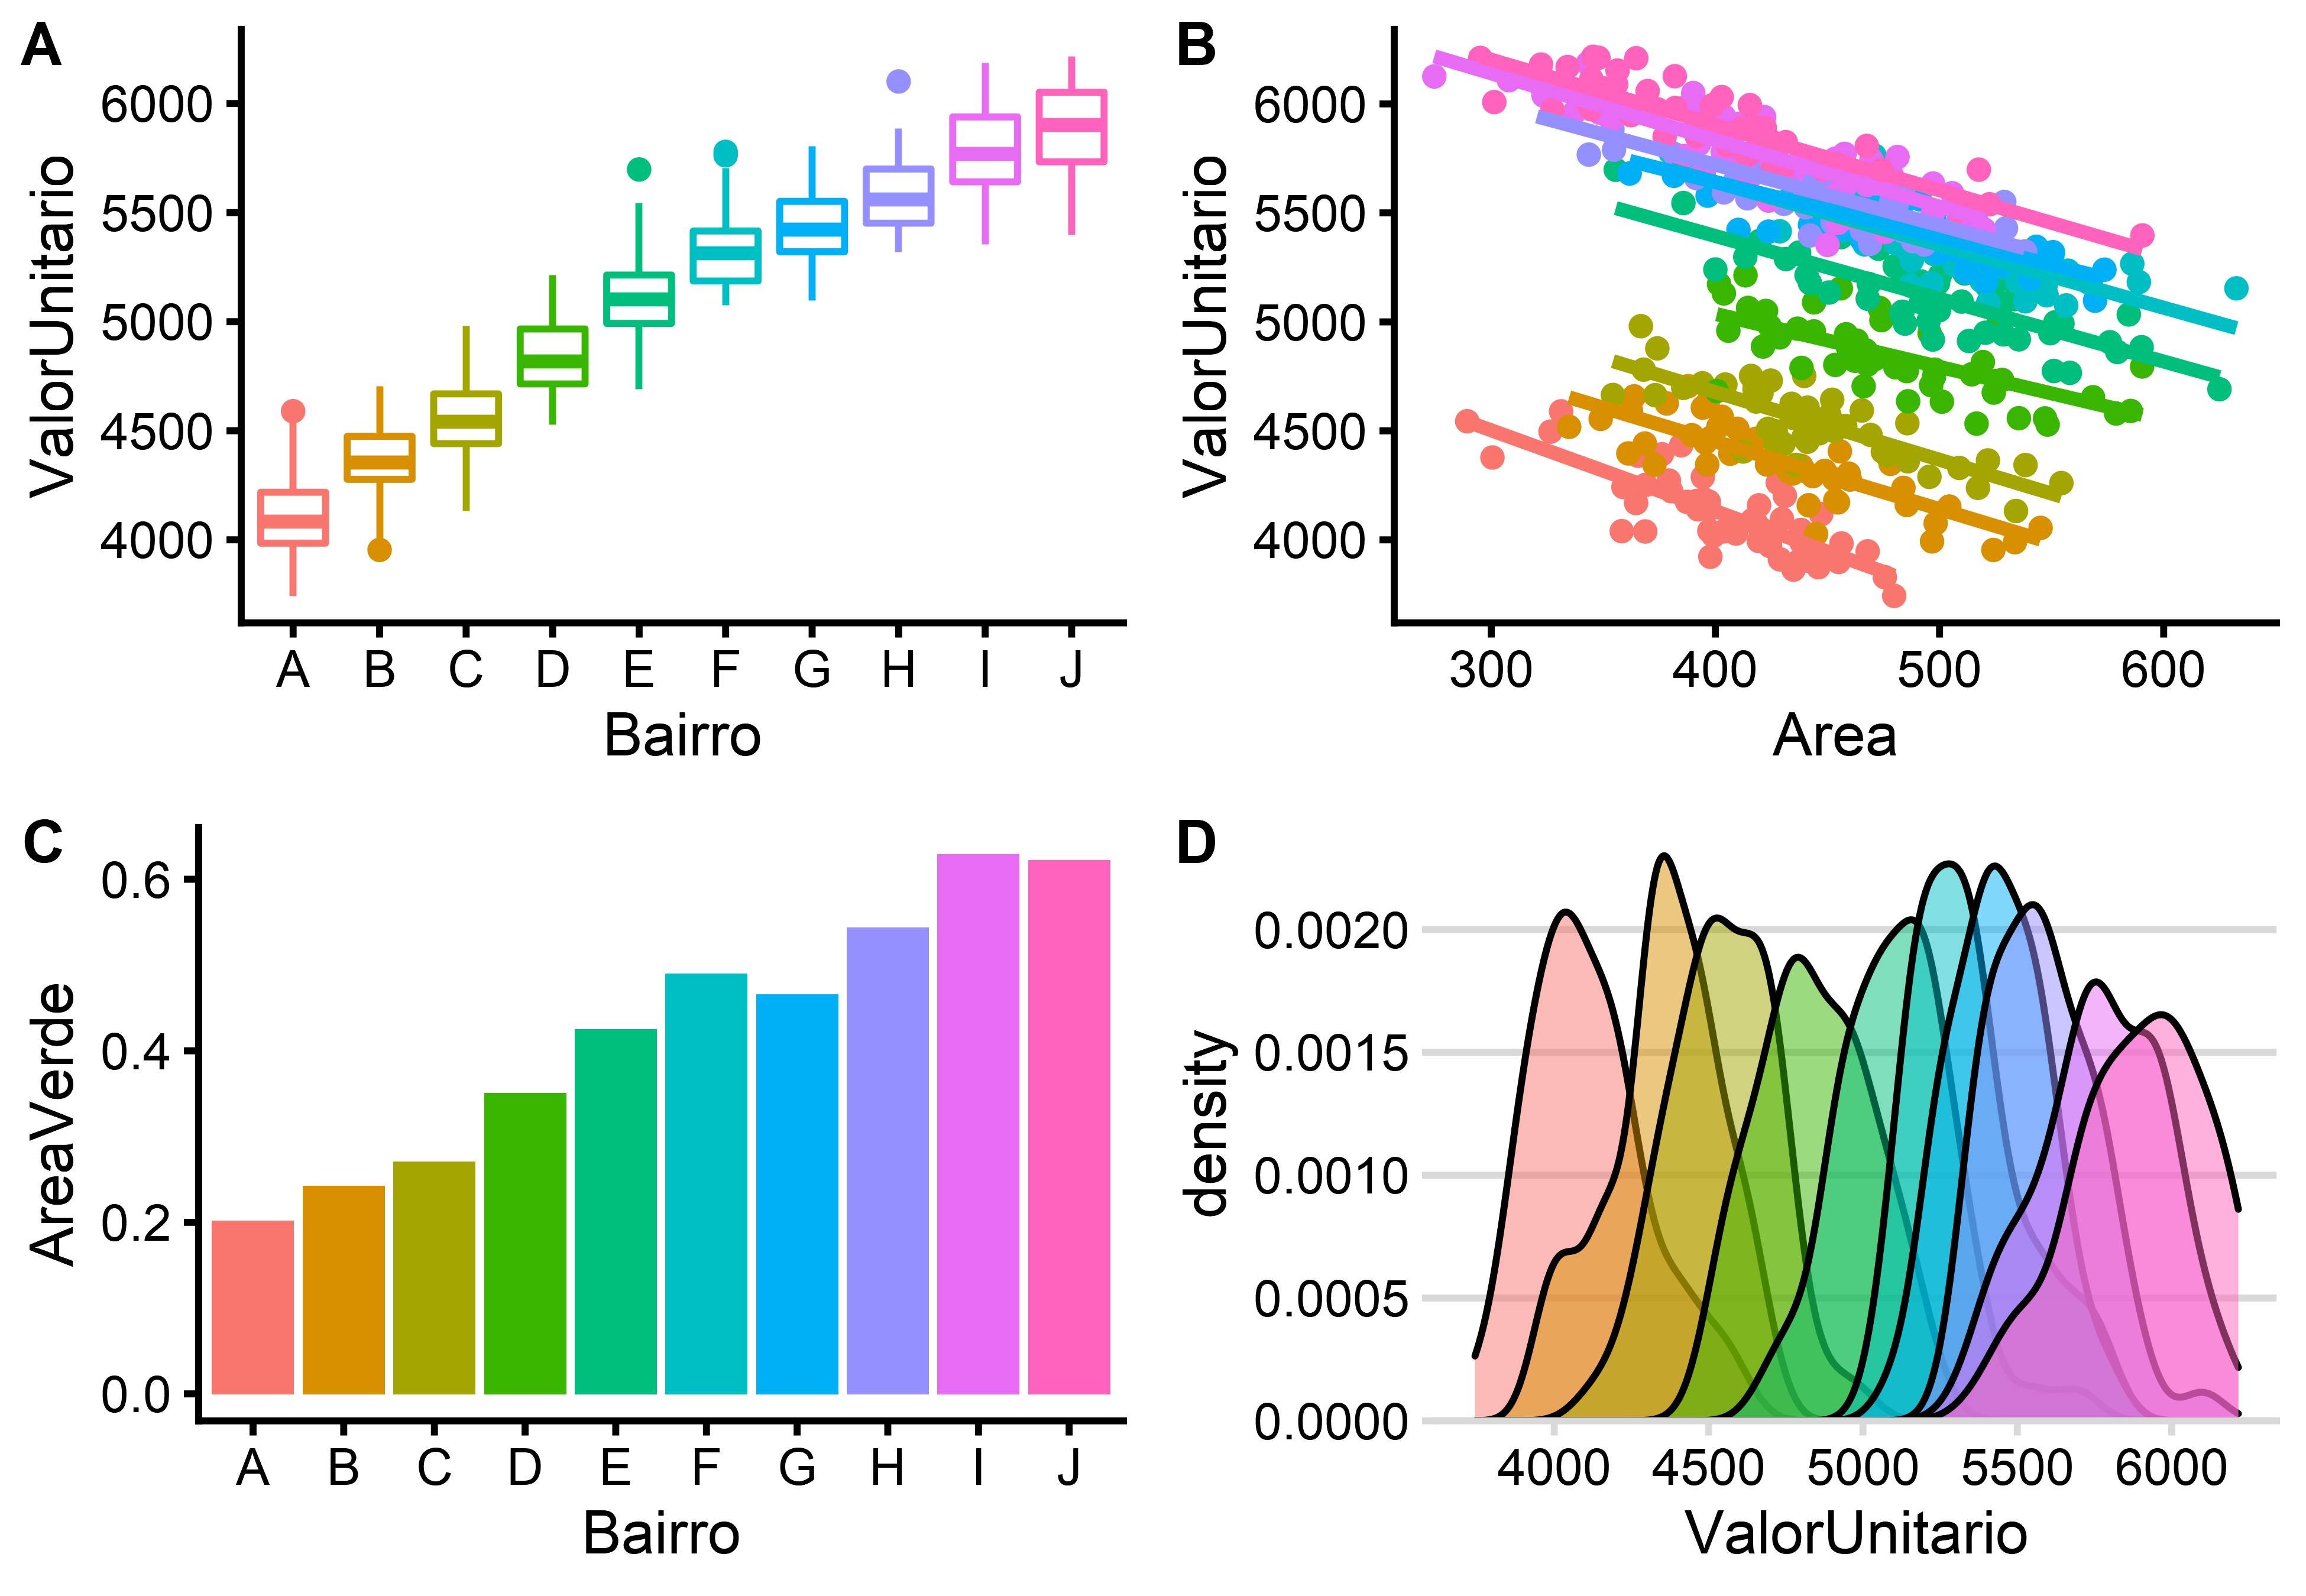
\includegraphics[width=1\linewidth]{images/exploratoria-1} 

}

\caption{Análise exploratória dos dados.}\label{fig:exploratoria}
\end{figure}

\hypertarget{ajuste-de-modelos}{%
\subsection{Ajuste de modelos}\label{ajuste-de-modelos}}

Com os dados gerados foram ajustados um modelo de efeitos fixos e três
modelos mistos: um modelo misto simples, que praticamente equivale ao
modelo de efeitos fixos, um modelo misto com a adição de uma variável de
segundo nível e um modelo misto utilizando-se a formulação de Mundlak.

Para o ajuste do modelo de efeitos fixos foram utilizados todos os dados
gerados, pois não há como prever valores para bairros não contemplados
na amostra em um modelo deste tipo.

\hypertarget{modelo-de-efeitos-fixos}{%
\subsubsection{Modelo de efeitos fixos}\label{modelo-de-efeitos-fixos}}

Com os dados gerados, foi elaborado um modelo de efeitos fixos sem
intercepto, apenas para que fique claro o valor do intercepto aleatório
de cada bairro. Para dar interpretação a estes interceptos aleatórios, a
variável \(Area\) foi centralizada em relação à área de um lote-padrão,
considerado de 400 \(m^2\)\footnote{A centralização de variáveis aqui
  presente não pretende nenhuma separação entre efeitos \emph{within} e
  \emph{between}, mas apenas possibilitar uma interpretação para os
  valores do coeficientes dos interceptos para cada bairro. Ver Droubi
  \emph{et al.} (\protect\hyperlink{ref-droubi2019}{2019}) para mais
  detalhes sobre este tipo de centralização.}

O modelo é descrito pela equação \ref{eq:fixefEC}:

\begin{equation} \label{eq:fixefEC}
ValorUnitario = \beta_1 (Area - 400) + \beta_{2j}Bairro_j + \varepsilon
\end{equation}

onde \(\beta_{2j}\) são os coeficientes das variáveis dicotômicas em
grupo (\(Bairro_j\)).

\hypertarget{modelos-mistos}{%
\subsubsection{Modelos mistos}\label{modelos-mistos}}

Para o ajuste dos modelos mistos foram removidos os 50 dados relativos
ao bairro H, que foram reservados para serem utilizados posteriormente
para validação dos modelos, mostrando como a previsão de valores em
modelos de efeitos mistos pode ser feita para agrupamentos não
contemplados na amostra.

\hypertarget{modelo-misto-simples}{%
\paragraph{Modelo misto simples}\label{modelo-misto-simples}}

Foi elaborado um modelo misto simples, sem separação de efeitos entre e
dentro dos agrupamentos, de acordo com a equação \ref{eq:simples}:

\begin{equation} \label{eq:simples}
ValorUnitario = \beta_0 + \beta_1 (Area - 400) + \upsilon_j + \varepsilon
\end{equation}

Onde \(\upsilon_j\) é uma variável aleatória que foi utilizada para
modelar os diferentes bairros.

\hypertarget{modelo-misto-com-variuxe1vel-de-segundo-nuxedvel}{%
\paragraph{Modelo misto com variável de segundo
nível}\label{modelo-misto-com-variuxe1vel-de-segundo-nuxedvel}}

Foi elaborado um modelo misto simples, porém com a presença de variáveis
de segundo nível hierárquico, como demonstrado na equação
\ref{eq:2ndlevel}:

\begin{equation} \label{eq:2ndlevel}
ValorUnitario = \beta_0 + \beta_1 (Area - 400) + \beta_2 A_{Vj}+ \upsilon_j + \varepsilon
\end{equation}

\hypertarget{modelo-misto-com-formulauxe7uxe3o-de-mundlak}{%
\paragraph{Modelo misto com formulação de
Mundlak}\label{modelo-misto-com-formulauxe7uxe3o-de-mundlak}}

Finalmente, foi ajusta um modelo com a formulação de Mundlak. Este
modelo foi elaborado de acordo com a formulação exibida na equação
\ref{eq:ECMundlak}:

\begin{equation} \label{eq:ECMundlak}
ValorUnitario = \beta_0 + \beta_1 Area + \beta_{1C} \overline{Area_j} + \beta_2 A_{Vj} + \upsilon_j + \varepsilon
\end{equation}

\hypertarget{resultados}{%
\subsection{Resultados}\label{resultados}}

A tabela \ref{tab:fits} mostra as estatísticas básicas dos diversos
modelos mistos (colunas 2, 3 e 4) comparados aos modelo de efeitos fixos
(coluna 1).

\begin{table}[H] \centering 
  \caption{Comparacão dos modelos de  efeitos fixos e efeitos mistos.} 
  \label{tab:fits} 
\scriptsize 
\begin{tabular}{@{\extracolsep{5pt}}lcccc} 
\\[-1.8ex]\hline 
\hline \\[-1.8ex] 
 & \multicolumn{4}{c}{\textit{Dependent variable:}} \\ 
\cline{2-5} 
\\[-1.8ex] & \multicolumn{4}{c}{ValorUnitario} \\ 
\\[-1.8ex] & \textit{OLS} & \multicolumn{3}{c}{\textit{linear}} \\ 
 & \textit{} & \multicolumn{3}{c}{\textit{mixed-effects}} \\ 
\\[-1.8ex] & (1) & (2) & (3) & (4)\\ 
\hline \\[-1.8ex] 
 Intercepto &  & 5.197,55 (216,47)$^{***}$ & 3.564,12 (188,59)$^{***}$ & 2.928,45 (371,57)$^{***}$ \\ 
  (Area - 400) & $-$2,92 (0,10)$^{***}$ & $-$2,94 (0,10)$^{***}$ & $-$2,92 (0,10)$^{***}$ &  \\ 
  Bairro A & 4.127,71 (15,39)$^{***}$ &  &  &  \\ 
  Bairro B & 4.445,83 (15,67)$^{***}$ &  &  &  \\ 
  Bairro C & 4.670,14 (15,92)$^{***}$ &  &  &  \\ 
  Bairro D & 5.075,49 (17,16)$^{***}$ &  &  &  \\ 
  Bairro E & 5.398,45 (18,08)$^{***}$ &  &  &  \\ 
  Bairro F & 5.645,72 (18,40)$^{***}$ &  &  &  \\ 
  Bairro G & 5.673,11 (17,23)$^{***}$ &  &  &  \\ 
  Bairro H & 5.728,11 (16,11)$^{***}$ &  &  &  \\ 
  Bairro I & 5.831,91 (15,49)$^{***}$ &  &  &  \\ 
  Bairro J & 5.903,05 (15,38)$^{***}$ &  &  &  \\ 
  Area &  &  &  & $-$2,94 (0,10)$^{***}$ \\ 
  Area (contexto) &  &  &  & 4,05 (0,81)$^{***}$ \\ 
  Area Verde &  &  & 3.975,12 (431,82)$^{***}$ & 3.940,15 (205,04)$^{***}$ \\ 
 \hline \\[-1.8ex] 
Observations & 500 & 450 & 450 & 450 \\ 
Log Likelihood &  & $-$2.781,80 & $-$2.764,57 & $-$2.758,14 \\ 
Akaike Inf. Crit. & 6.120,87 & 5.571,60 & 5.539,13 & 5.528,27 \\ 
Bayesian Inf. Crit. & 6.171,44 & 5.588,04 & 5.559,68 & 5.552,93 \\ 
\hline 
\hline \\[-1.8ex] 
\textit{Note:}  & \multicolumn{4}{r}{$^{*}$p$<$0,3; $^{**}$p$<$0,2; $^{***}$p$<$0,1} \\ 
\end{tabular} 
\end{table}

Deve-se notar, primeiramente, que os valores estimados pelo modelo de
efeitos fixos para os interceptos de cada bairro (coluna 1 da tabela
\ref{tab:fits}) são praticamente os mesmos valores obtidos pela
estimação do modelo misto simples, descritos na tabela
\ref{tab:somaitcpt}, onde os valores de referência para cada bairro
foram obtidos através da soma do intercepto global do modelo misto
simples com os interceptos aleatórios do modelo misto simples, que podem
ser visualizados na Figura \ref{fig:dotplot}. A única exceção é o bairro
H, que foi suprimido da amostra para a confecção do modelo misto.

Como se pode notar na Figura \ref{fig:dotplot}, os valores dos
interceptos aleatórios para cada bairro giram em torno de zero, o seu
valor médio. Como o Bairro H (com \(A_V = 0,55\)) foi omitido no ajusto
do modelo, não há valores estimados para os efeitos aleatórios para este
bairro.

A ínica informação a mais que se pode extrair do modelo de efeitos
mistos simples é a componente de variância devido à localidade, separada
da variância ao nível dos imóveis, o que pode ser visto na tabela
\ref{tab:variancias}.

\begin{table}[H]

\caption{\label{tab:somaitcpt}Valores dos interceptos para cada bairro.}
\centering
\fontsize{10}{12}\selectfont
\begin{tabular}[t]{rrrrrrrrr}
\toprule
A & B & C & D & E & F & G & I & J\\
\midrule
4.128,4 & 4.446,7 & 4.671 & 5.076,7 & 5.399,7 & 5.646,9 & 5.674 & 5.831,8 & 5.902,7\\
\bottomrule
\end{tabular}
\end{table}

\begin{table}[H]

\caption{\label{tab:variancias}Efeitos randômicos do modelo misto.}
\centering
\begin{tabular}[t]{lrr}
\toprule
grp & vcov & sdcor\\
\midrule
\cellcolor{gray!6}{Bairro} & \cellcolor{gray!6}{421.256,03} & \cellcolor{gray!6}{649,04}\\
Residual & 12.123,29 & 110,11\\
\bottomrule
\end{tabular}
\end{table}

\begin{figure}[H]

{\centering 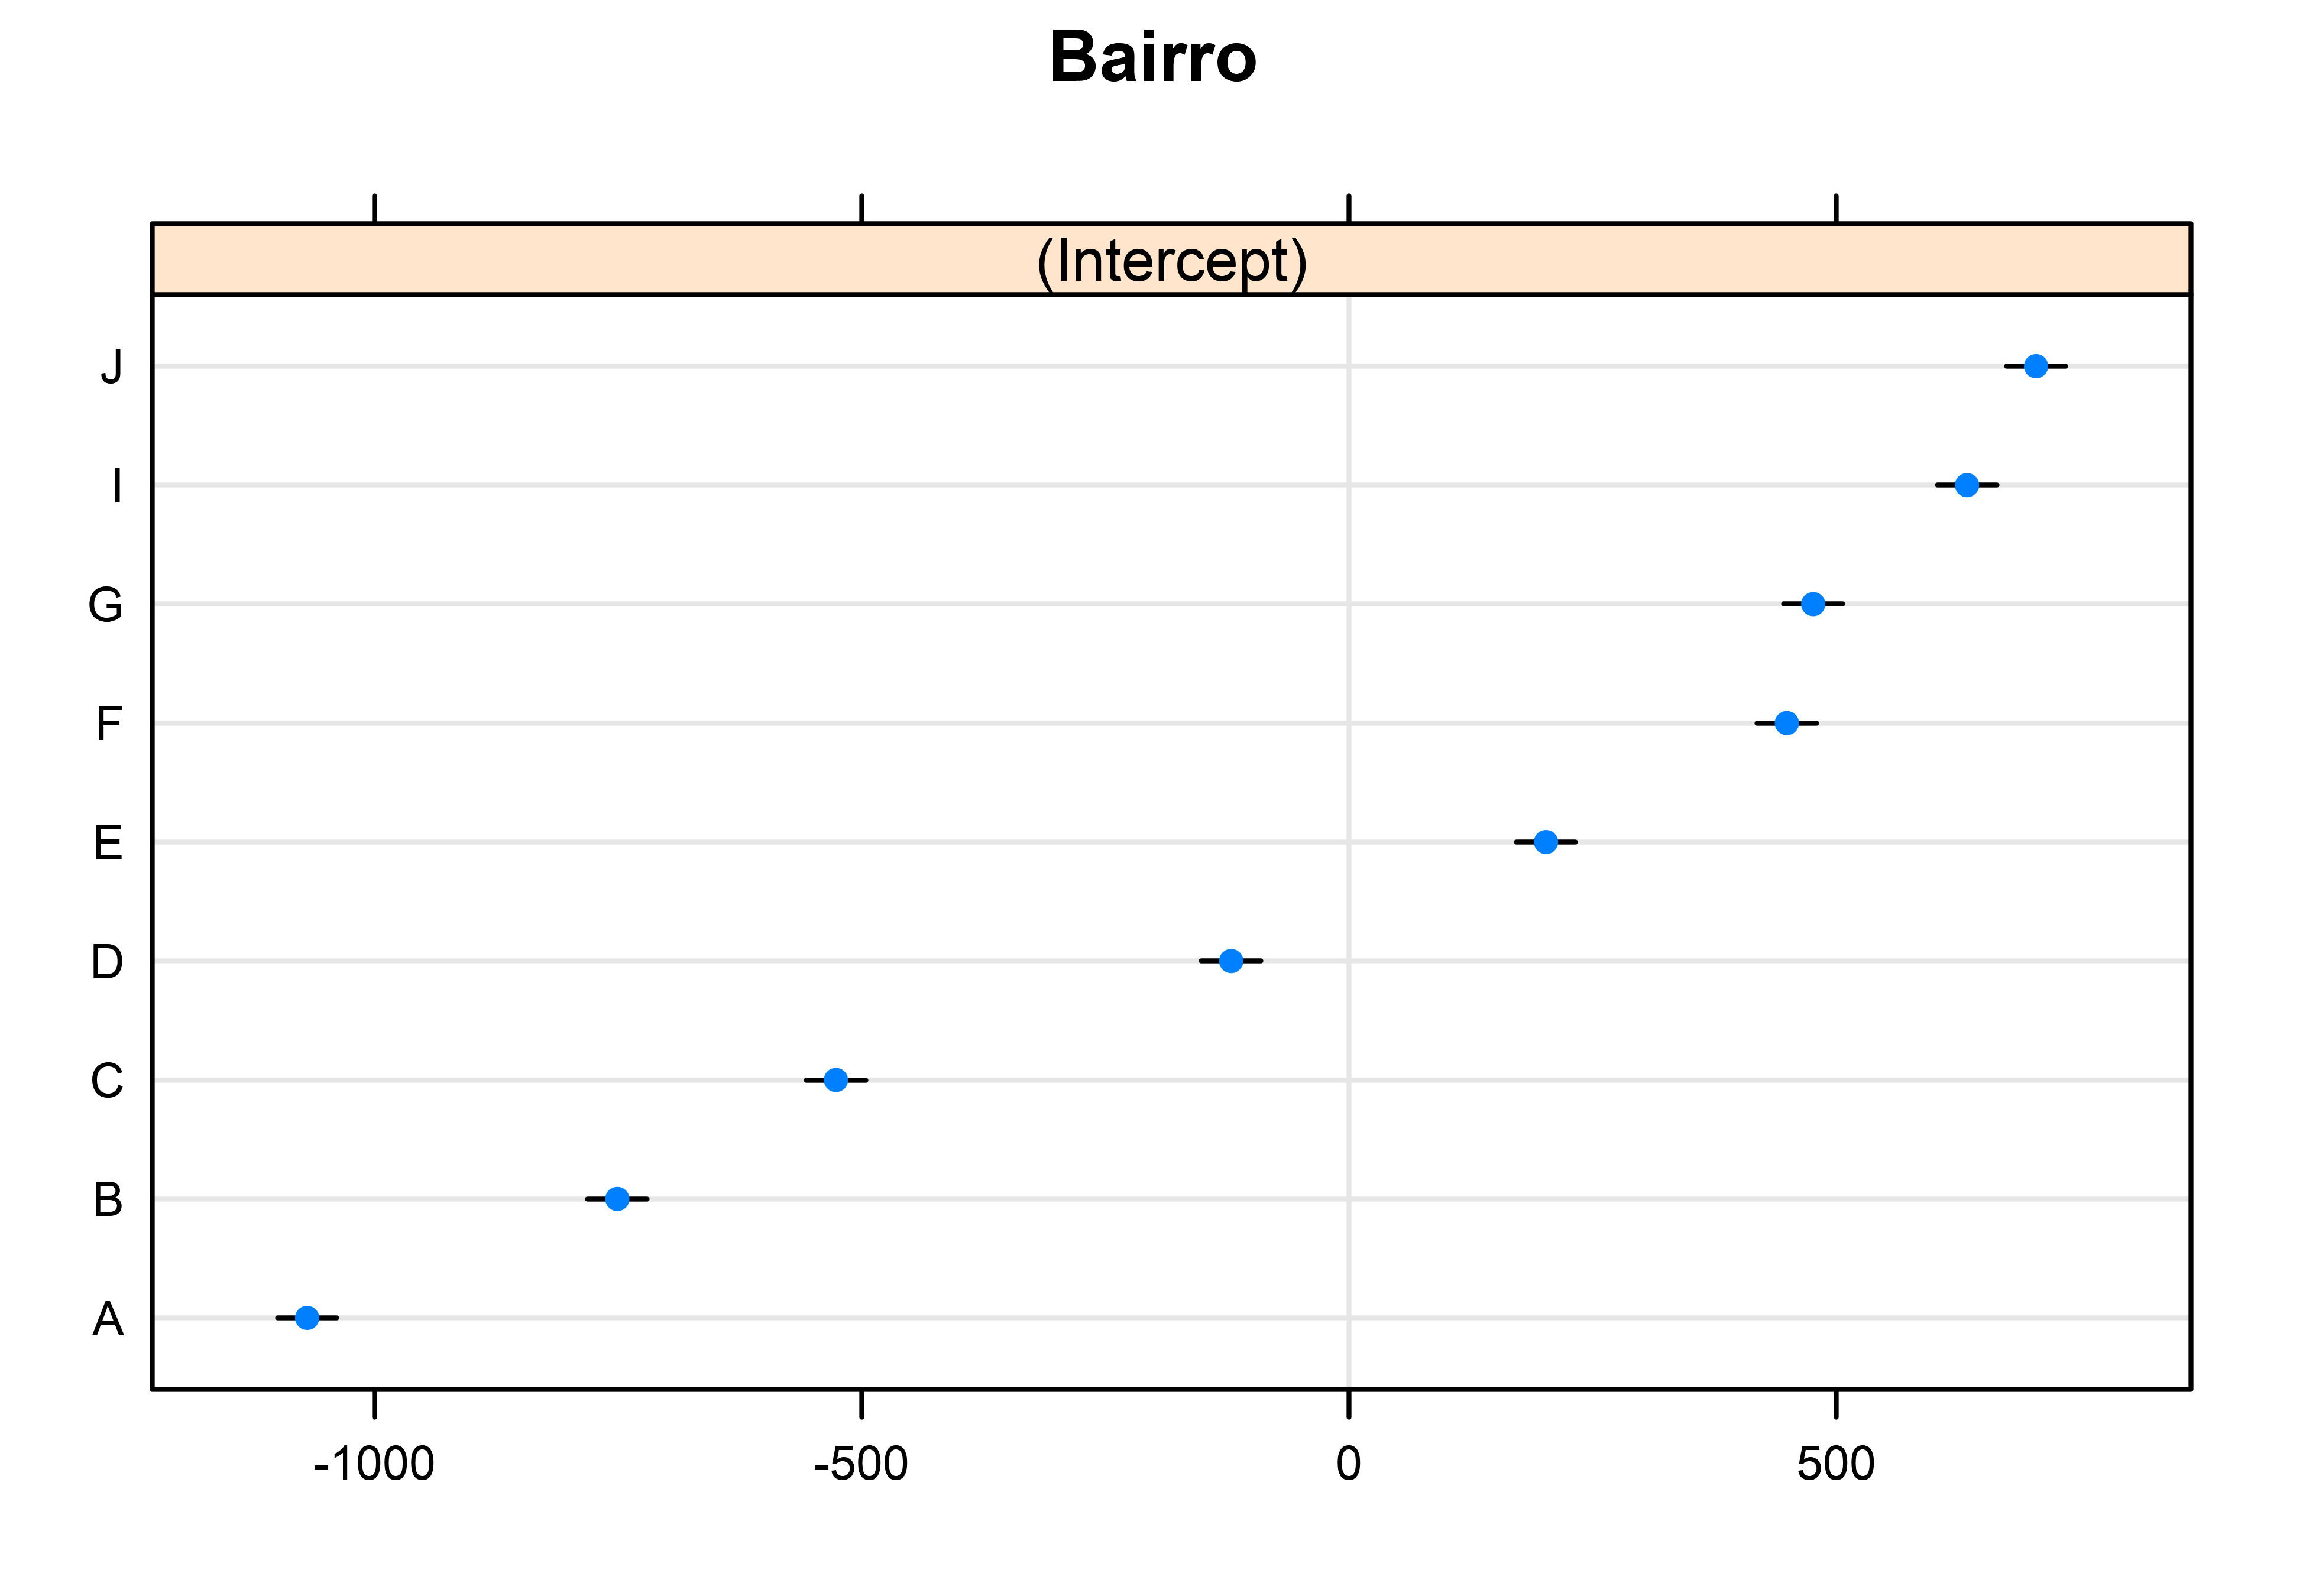
\includegraphics[width=0.7\linewidth]{images/dotplot-1} 

}

\caption{Efeitos aleatórios do modelo.}\label{fig:dotplot}
\end{figure}

Pode-se notar que a variância devido à localidade é relevante para o
modelo, haja vista que a variância devido à localidade é maior do que a
variância devido às características dos imóveis.

Nos modelos onde houve a inclusão da variável Área Verde (\(A_V\)), seu
coeficiente foi bem estimado: o valor da influência das áreas verdes,
simulado como aumento R\$ 40,00/m2 a cada ponto percentual a mais de
áreas verdes no bairro do imóvel, foi precisamente estimado.

Para o modelo de Mundlak, a estimação do coeficiente contextual
(\(\beta_{1C}\)) também resultou significante, conforme esperado, já que
os dados foram gerados com áreas médias diferentes para cada bairro.

Deve-se ponderar que, caso os dados não tivessem a estrutura esperada
para a formulação adotada, haveria degeneração dos modelos. Por exemplo,
caso não houvesse de fato variância alguma entre os bairros, ou seja, se
o pertencimento a um determinado agrupamento não afetar na formação
final de preços, o valor estimado para o desvio-padrão do efeito
aleatório \(\upsilon\) seria igual a zero, \emph{i. e.}
\(\hat \sigma_\upsilon = 0\) (BATES,
\protect\hyperlink{ref-Batesbook}{2010}, pp. 10--11) situação em que o
modelo misto degenera para um modelo de regressão linear ordinária. No
caso da formulação de Mundlak, caso não houvesse o efeito contextual, a
variável de contexto não apresentaria significância, ou seja, deveria
ser removida do modelo, fazendo com que o modelo degenere para um modelo
misto simples.

Outra maneira de se testar a pertinência da formulação de Mundlak seria
através da Análise de Variância. A tabela \ref{tab:anova} faz a
comparação entre o modelo de efeitos mistos sem variáveis de segundo
nível (primeira linha), com a variável de segundo nível \(A_V\) (segunda
linha) e com a formulação de Mundlak (terceira linha). Percebe-se que é
significante a melhora advinda da adição de um novo parâmetro no segundo
modelo, assim como também é significante a adoção de um novo parâmetro
pela formulação de Mundlak, o que se nota nos baixos p-valores
constantes da última coluna (zero).

\begin{table}

\caption{\label{tab:anova}Análise de Variância.}
\centering
\begin{tabular}[t]{lrrrrrrrr}
\toprule
  & npar & AIC & BIC & logLik & deviance & Chisq & Df & Pr(>Chisq)\\
\midrule
\cellcolor{gray!6}{fit\_lmer} & \cellcolor{gray!6}{4} & \cellcolor{gray!6}{5.581,43} & \cellcolor{gray!6}{5.597,86} & \cellcolor{gray!6}{-2.786,71} & \cellcolor{gray!6}{5.573,43} & \cellcolor{gray!6}{NA} & \cellcolor{gray!6}{NA} & \cellcolor{gray!6}{NA}\\
fit\_lmer2 & 5 & 5.560,28 & 5.580,83 & -2.775,14 & 5.550,28 & 23,15 & 1 & 0\\
\cellcolor{gray!6}{mundlak} & \cellcolor{gray!6}{6} & \cellcolor{gray!6}{5.547,46} & \cellcolor{gray!6}{5.572,12} & \cellcolor{gray!6}{-2.767,73} & \cellcolor{gray!6}{5.535,46} & \cellcolor{gray!6}{14,82} & \cellcolor{gray!6}{1} & \cellcolor{gray!6}{0}\\
\bottomrule
\end{tabular}
\end{table}

Por último, porém não menos relevante, percebe-se que este modelo tem
critérios de informação de Akaike (AIC) e de Bayes (BIC) melhores que os
dois modelos iniciais.

Nas Figuras \ref{fig:pr}, \ref{fig:pr1} e \ref{fig:pr2} podem ser vistos
os gráficos de densidades para os parâmetros estimados pelos modelos de
efeitos mistos simples, com variável de segundo nível e com formulação
de Mundlak, respectivamente. Nota-se que a ausência da variável de
segundo nível levou o modelo de efeitos mistos simples a uma má
estimação da distribuição da variável \(\sigma_\upsilon\) (no gráfico
\(\sigma_1\)), que apresentou uma longa cauda, com valores possíveis
entre aproximadamente 400 e 1400.

Com o acréscimo da variável de segundo nível esta variável ficou com
magnitude bem menor, ou seja, a introdução da variável de segundo nível
reduziu a variação não-explicada pelo modelo. Por fim, a introdução da
variável contextual reduziu ainda mais a variação não-explicada, gerando
uma estimação precisa da variância do termo aleatório
\(\sigma_\upsilon\).

\begin{figure}[H]

{\centering 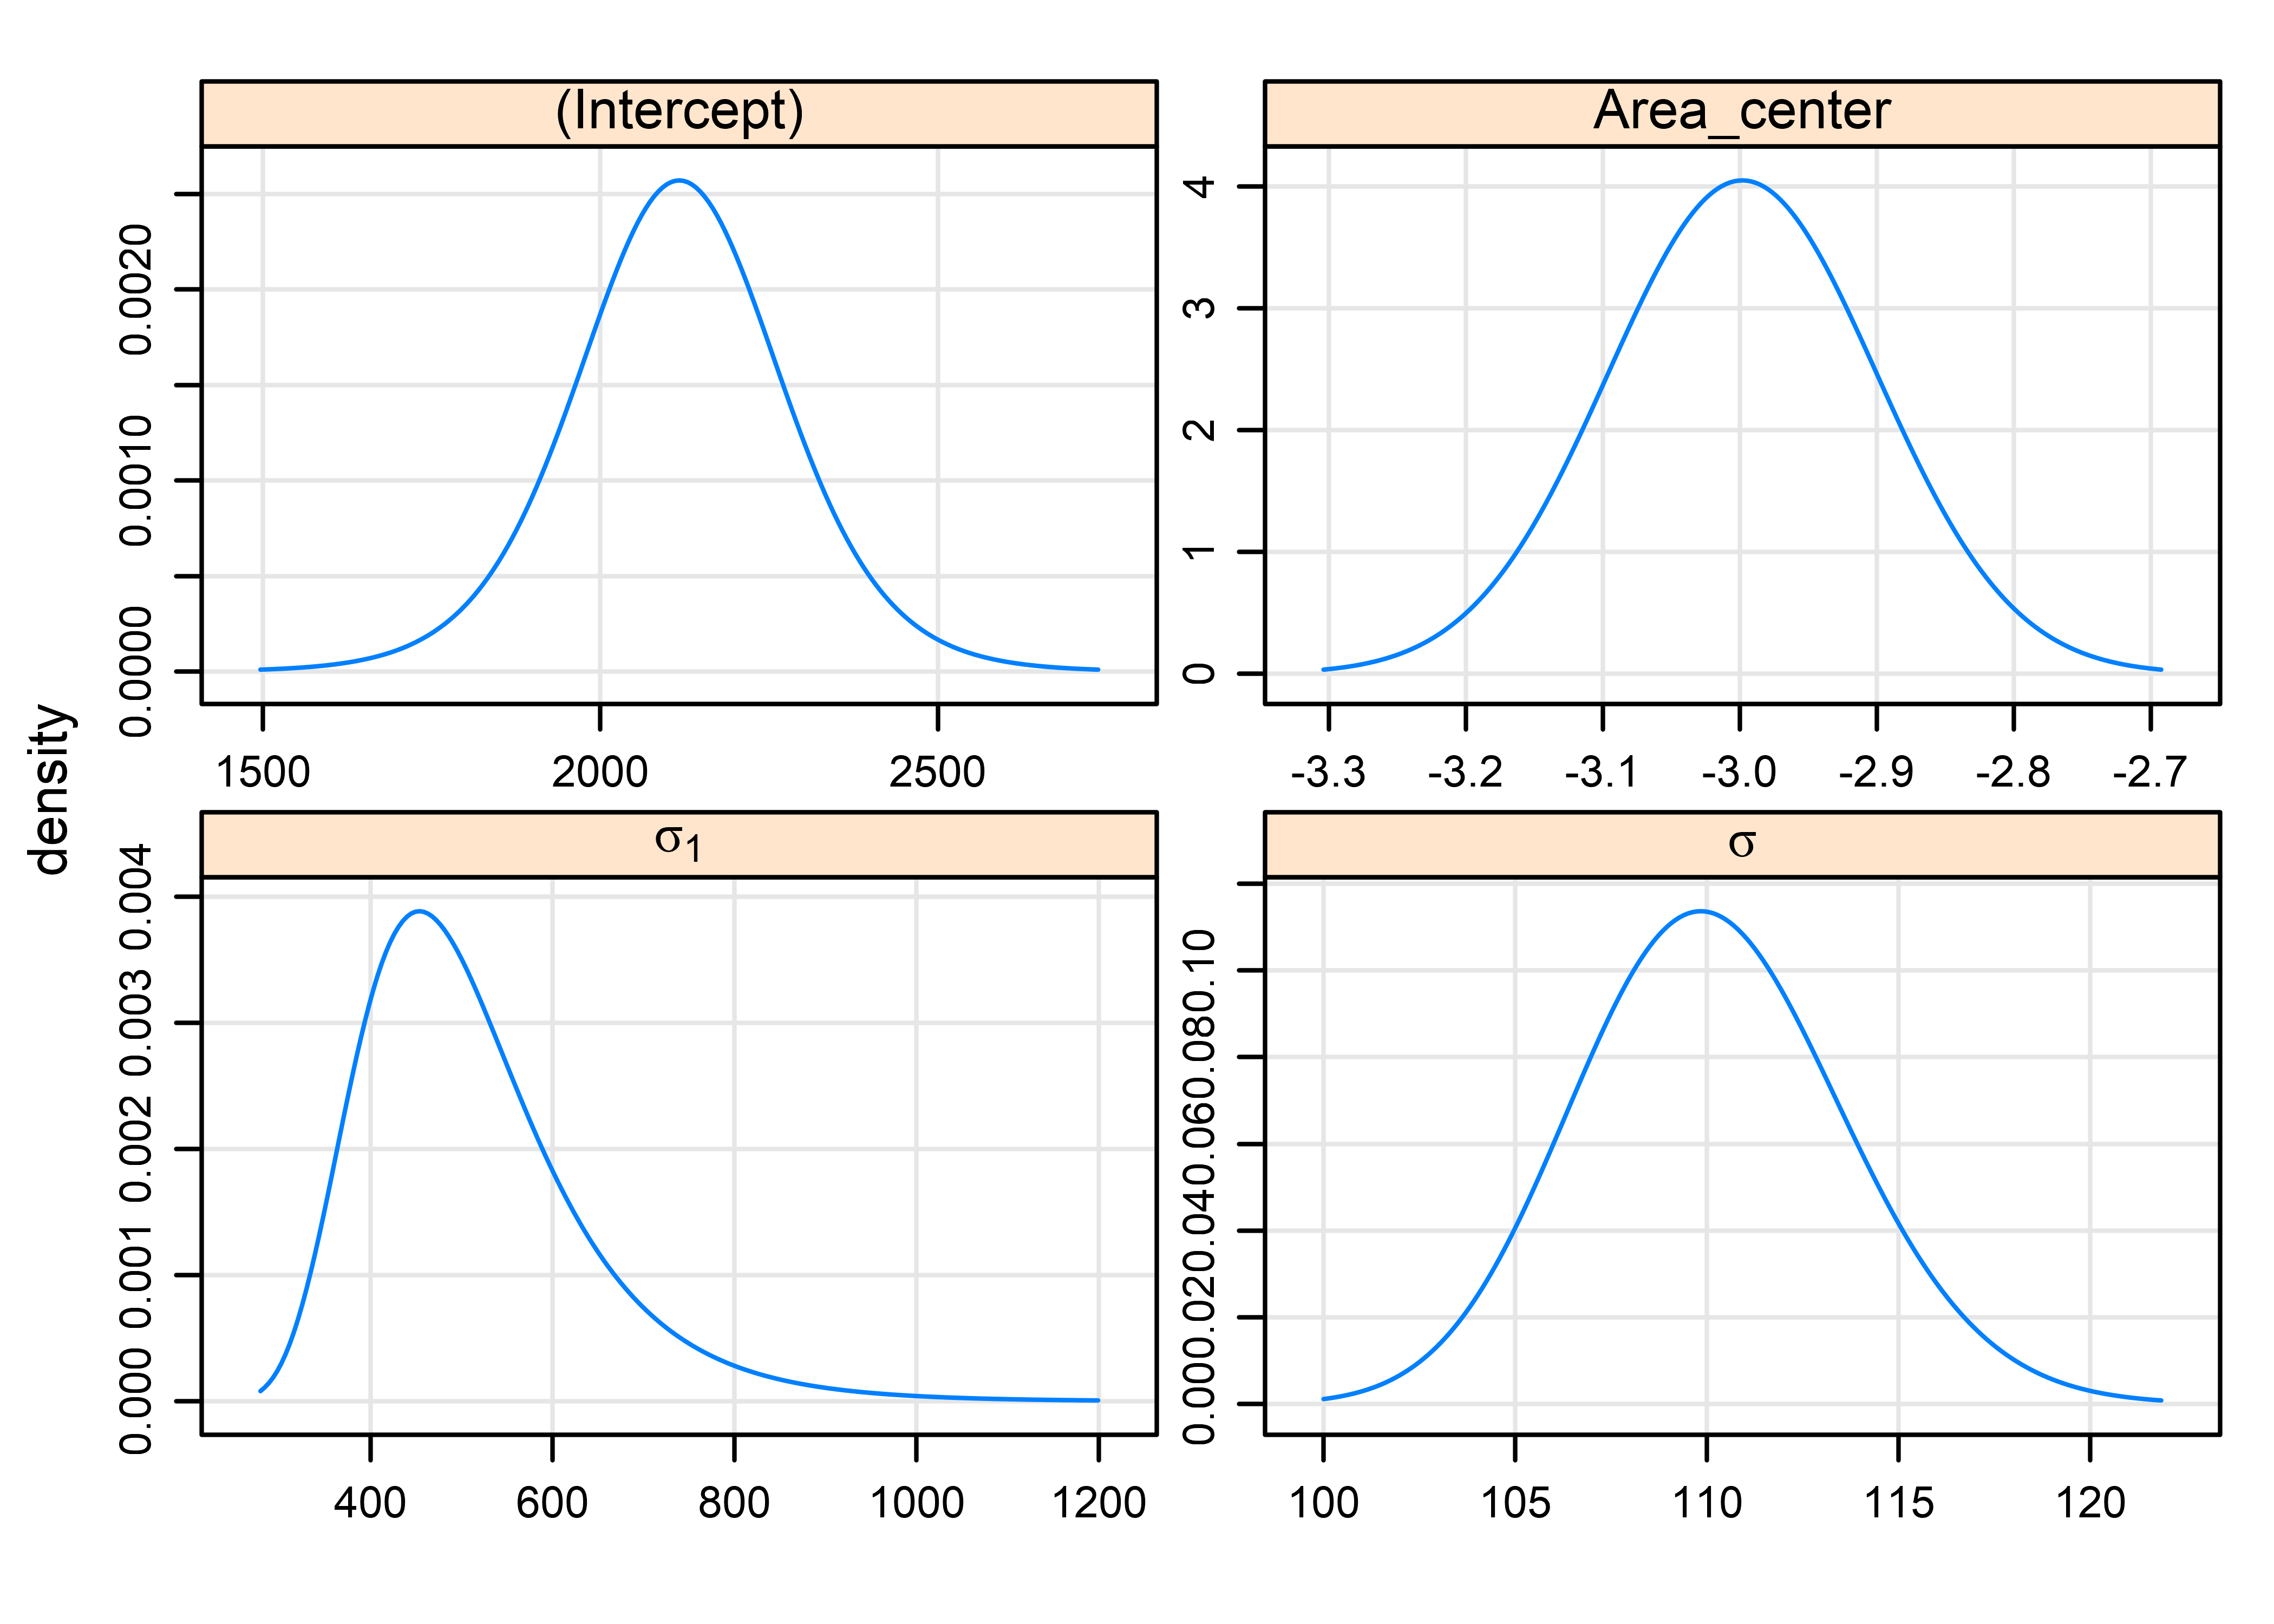
\includegraphics[width=0.5\linewidth]{images/pr-1} 

}

\caption{Densidades dos parâmetros do modelo de efeitos mistos simples.}\label{fig:pr}
\end{figure}

\begin{figure}[H]

{\centering 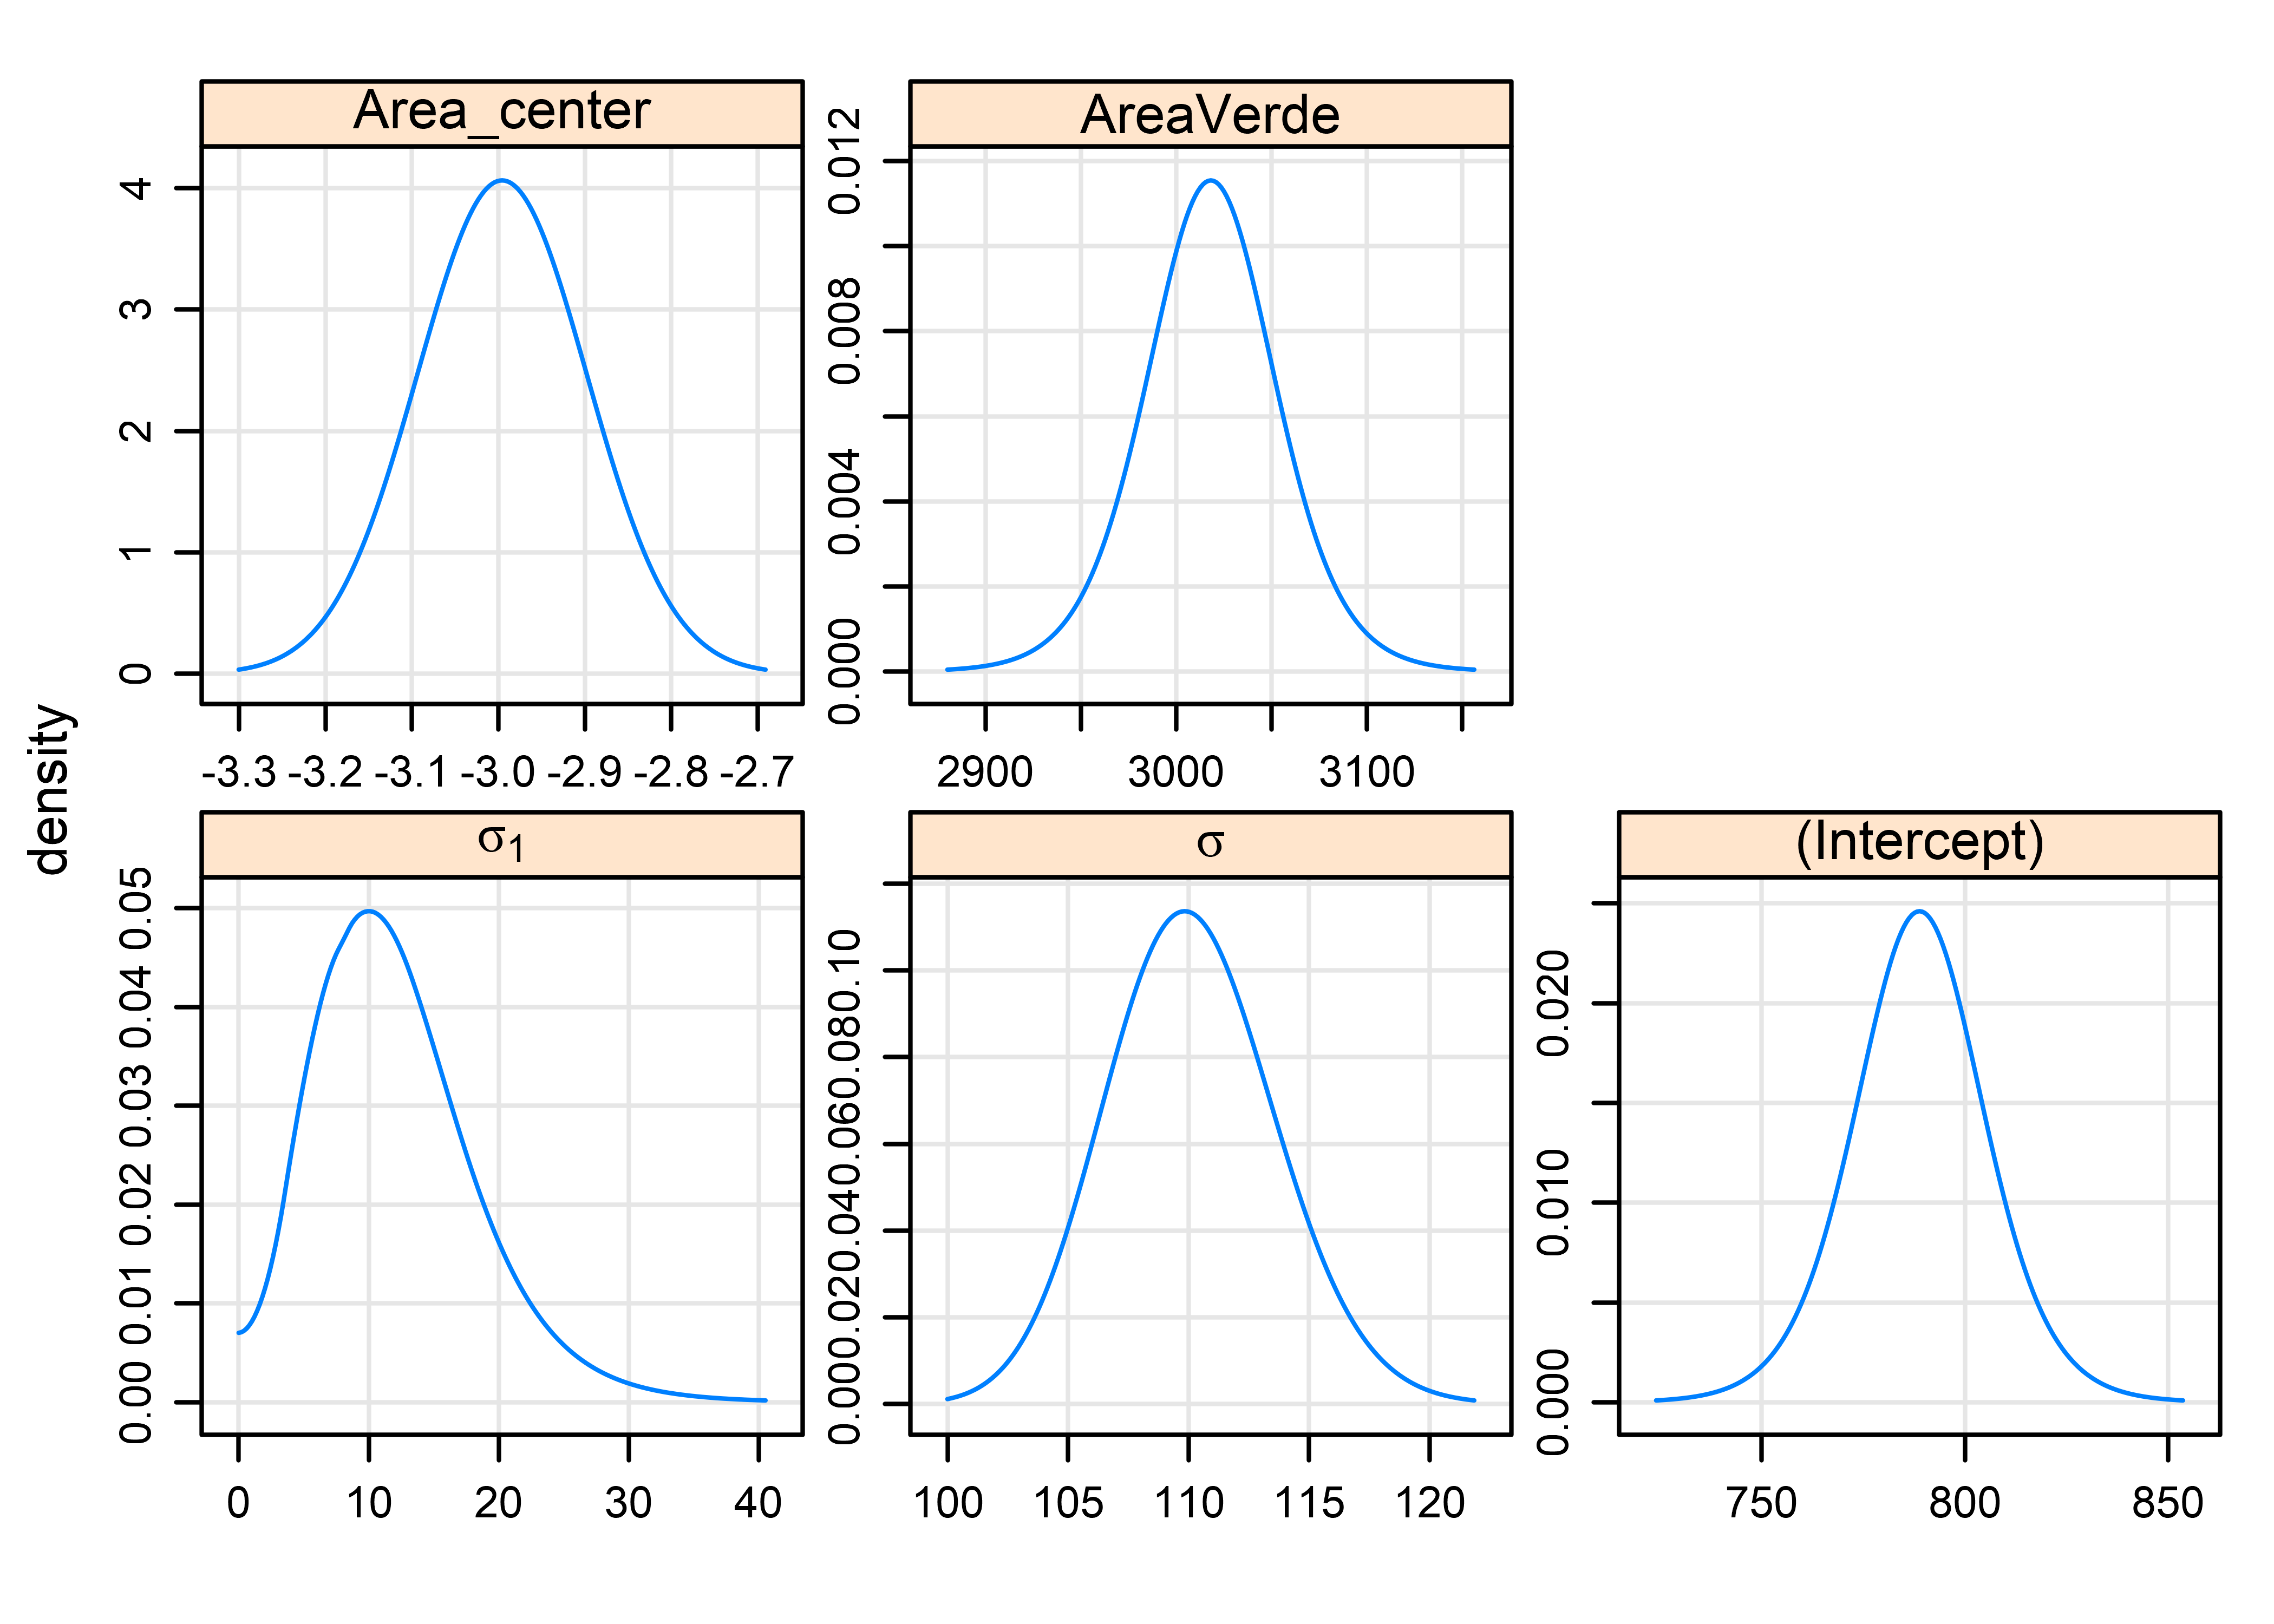
\includegraphics[width=0.75\linewidth]{images/pr1-1} 

}

\caption{Densidades dos parâmetros do modelo de efeitos mistos com variável de segundo nível.}\label{fig:pr1}
\end{figure}
\begin{figure}[H]

{\centering 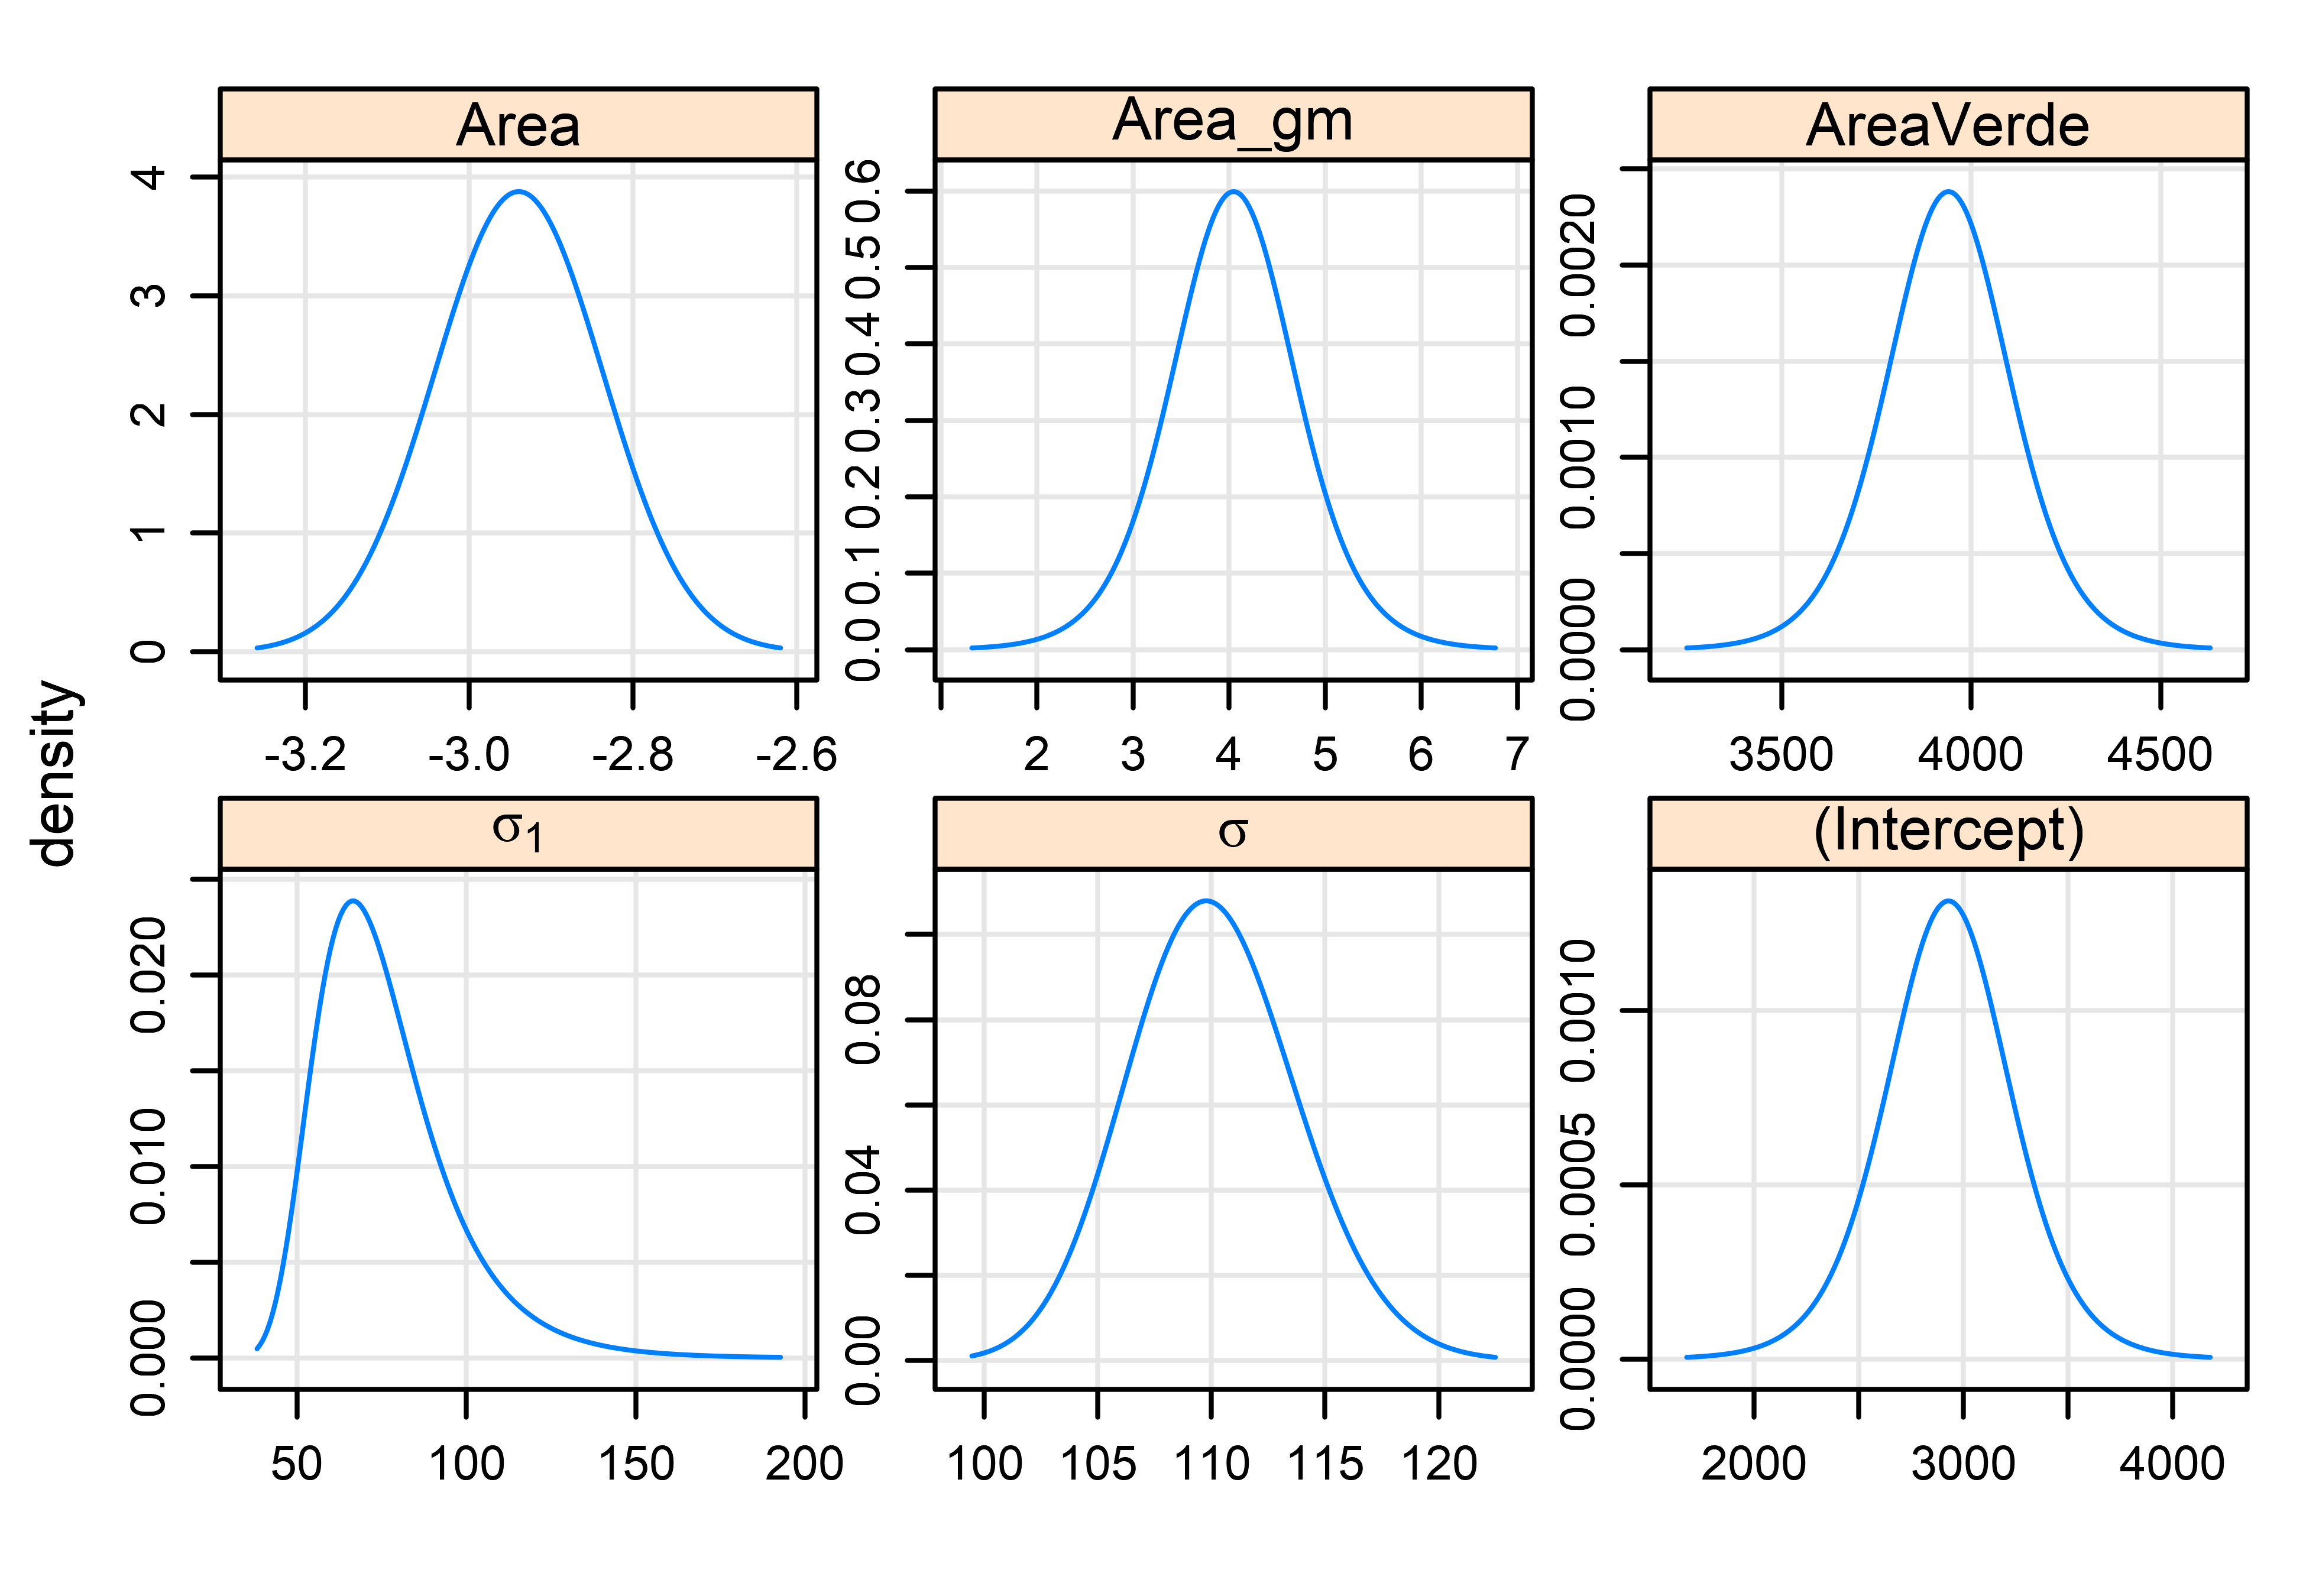
\includegraphics[width=0.75\linewidth]{images/pr2-1} 

}

\caption{Densidades dos parâmetros do modelo de Mundlak.}\label{fig:pr2}
\end{figure}

\hypertarget{previsuxe3o-de-valores}{%
\subsection{Previsão de Valores}\label{previsuxe3o-de-valores}}

Para ilustrar como os modelos mistos podem ser utilizados no contexto de
predição, foram elaboradas previsões no bairro H, que havia sido
propositalmente excluído no ajuste dos modelos mistos, com os diversos
modelos apresentados.

Também foram utilizados o modelo de efeitos fixos e o modelo misto com a
variável de segundo nível \(A_V\) para a previsão de valores de
lote-padrão para os diversos bairros, inclusive para o bairro H, não
utilizado para a confecção dos modelos mistos.

\hypertarget{previsuxe3o-de-dados-no-bairro-h}{%
\subsubsection{Previsão de dados no bairro
H}\label{previsuxe3o-de-dados-no-bairro-h}}

Na Figura \ref{fig:powerPlots} podem ser vistos os gráficos de poder de
predição para o modelo de efeitos fixos (A), para o modelo misto simples
(B), para o modelo misto com a variável de segundo nível (C) e para o
modelo misto com formulação de Mundlak (D). Como pode ser visto, todos
os modelos possuem poderes de predição praticamente equivalentes, com
exceção do modelo misto simples, onde a previsão de valores não pode ser
feita com precisão já que, como no modelo de efeitos fixos, este modelo
não tem parâmetros para prever valores em bairros não contemplados na
amostra. Para efetuar as previsões no bairro H, então, o modelo
considerou para a variável aleatória \(\upsilon\) o valor zero, ou seja,
o valor esperado da variável, o que levou a previsões incorretas em
relação aos valores simulados para aquele bairro.

\begin{figure}[H]

{\centering 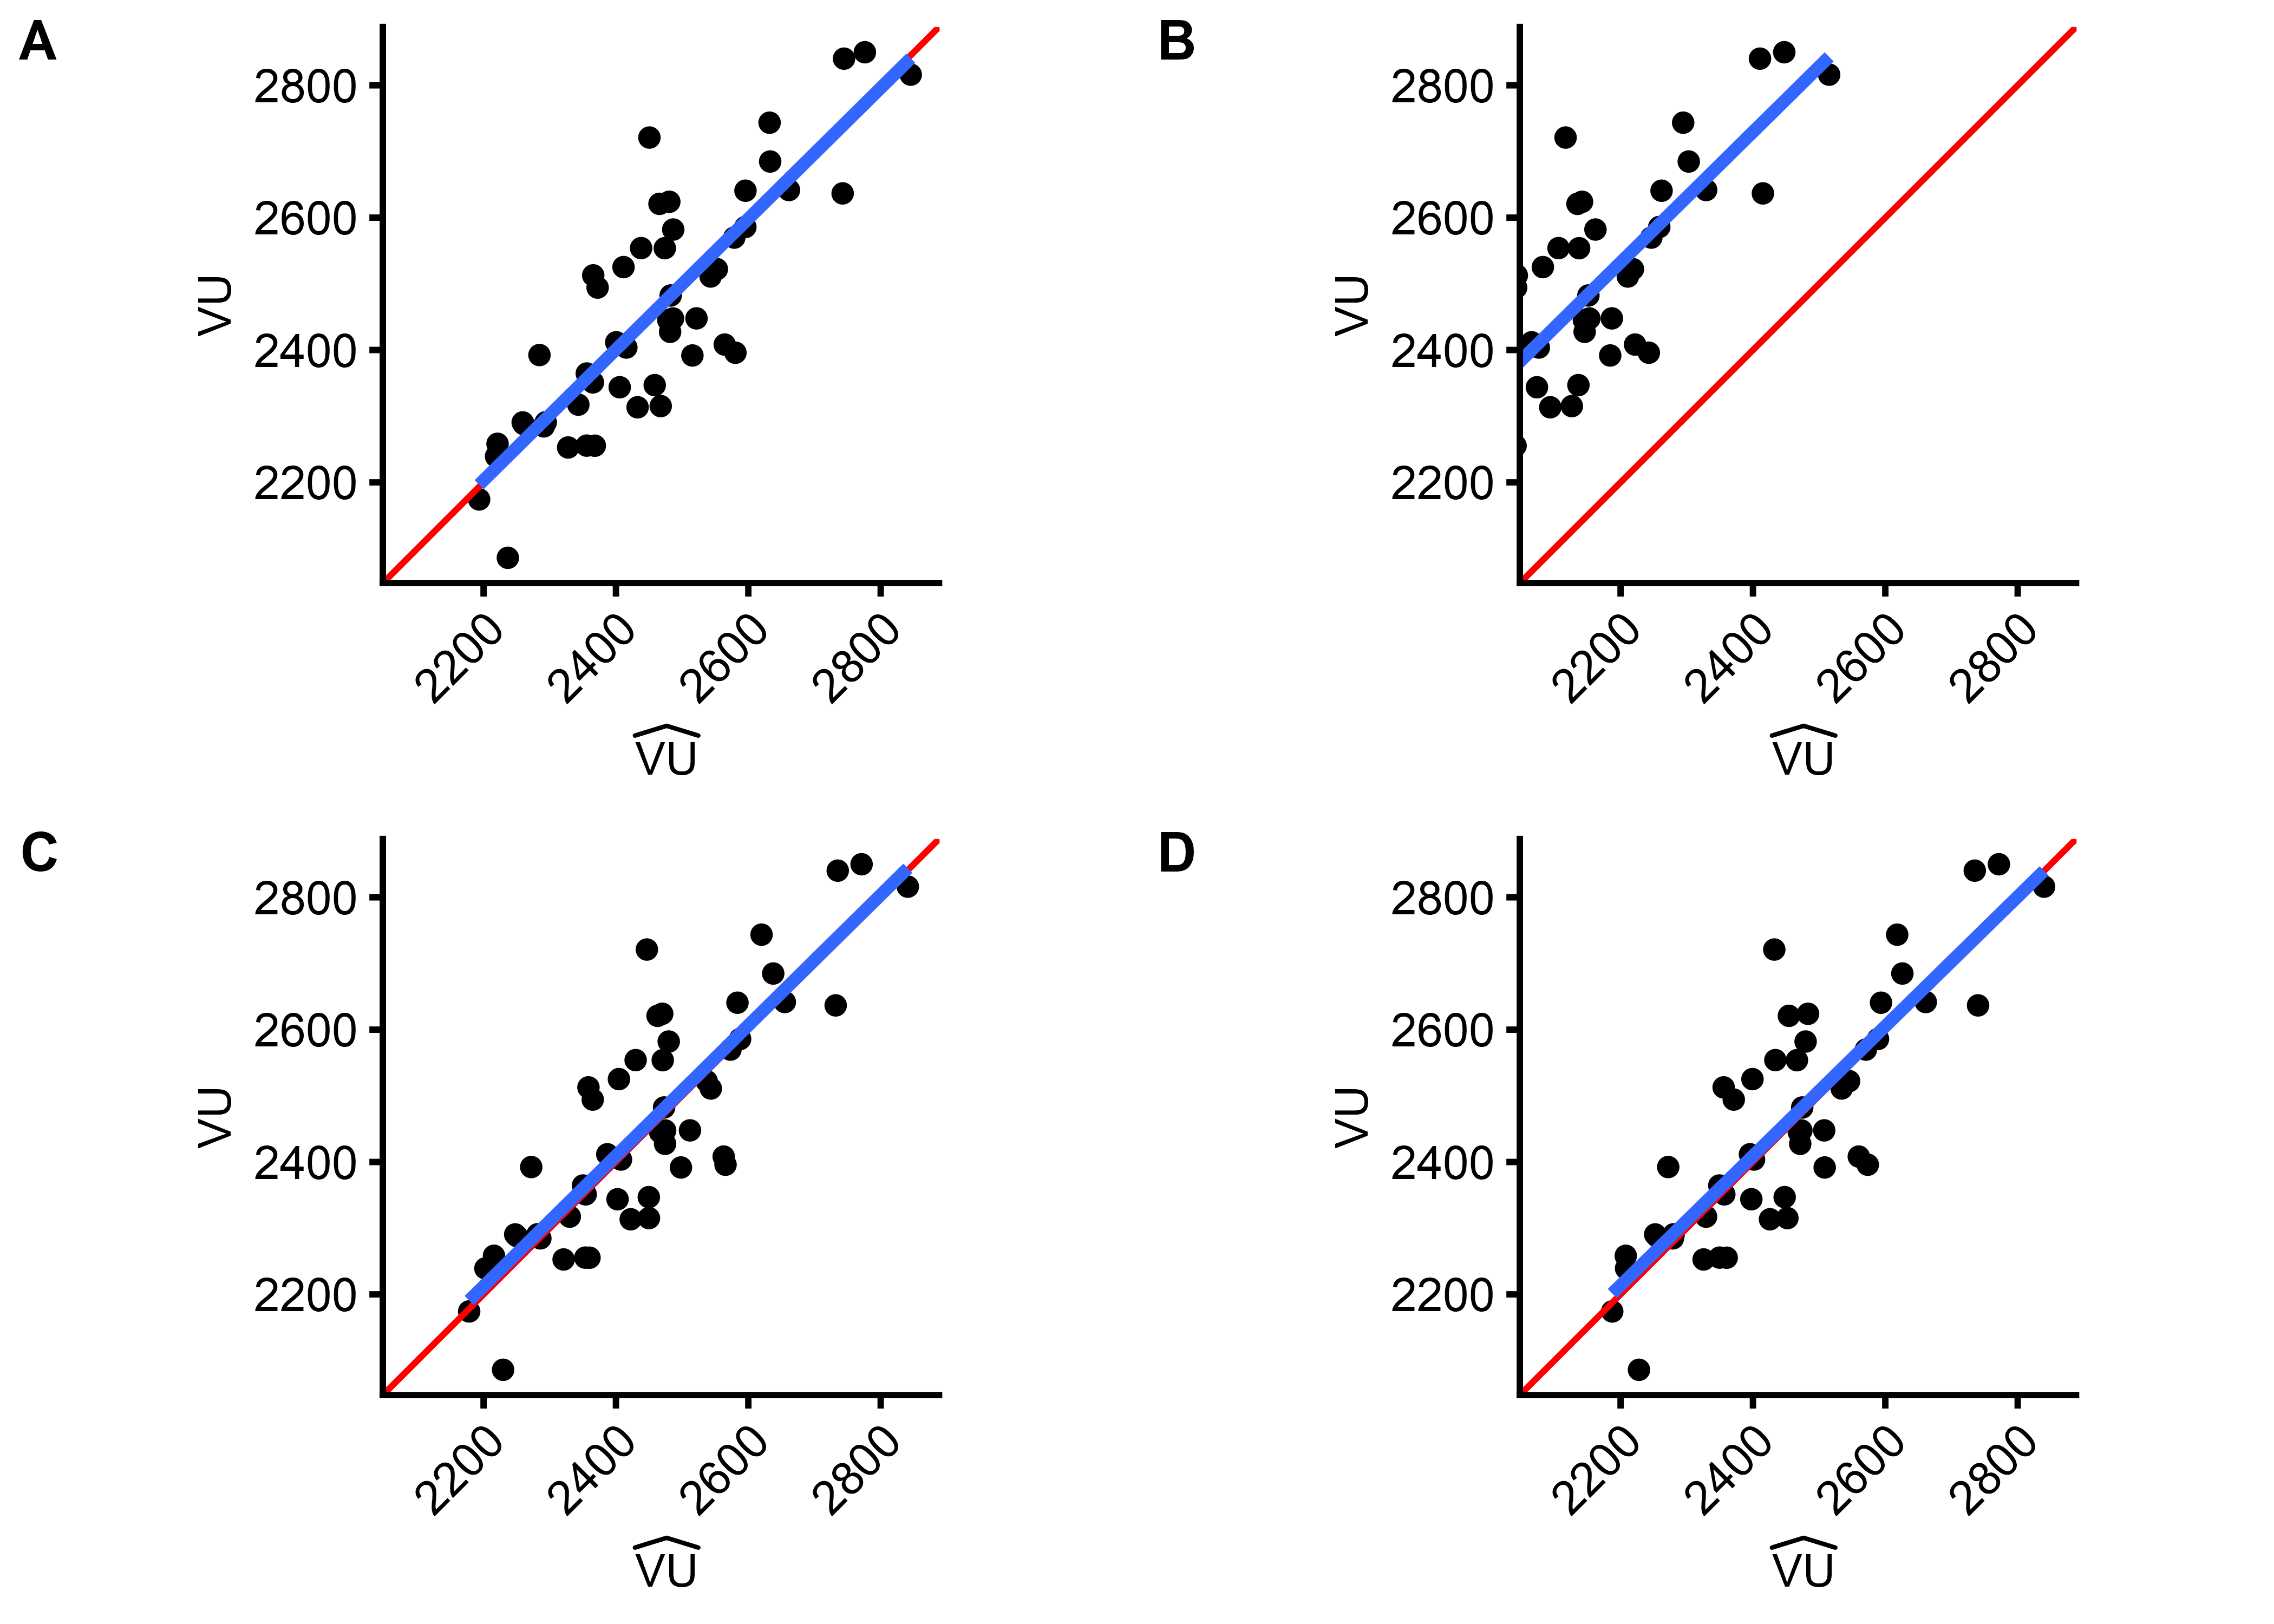
\includegraphics[width=1\linewidth]{images/powerPlots-1} 

}

\caption{Gráficos de poder de predição para cada modelo.}\label{fig:powerPlots}
\end{figure}

\hypertarget{previsuxe3o-de-valores-para-lotes-padruxe3o}{%
\subsubsection{Previsão de valores para
lotes-padrão}\label{previsuxe3o-de-valores-para-lotes-padruxe3o}}

Assim como a previsão de valores para os dados simulados para o bairro
H, conforme se mostrou no item anterior, é possível prever valores para
um lote-padrão nos diferentes bairros.

A tabela abaixo mostra os valores previsto pelos modelos para um
lote-padrão de 400 \(m^2\) nos diversos bairros:

\begin{longtable}[]{@{}cccc@{}}
\caption{Previsões para valores de lote-padrão nos diferentes
bairros.}\tabularnewline
\toprule
\begin{minipage}[b]{0.06\columnwidth}\centering
Bairro\strut
\end{minipage} & \begin{minipage}[b]{0.35\columnwidth}\centering
Modelo de efeitos fixos\strut
\end{minipage} & \begin{minipage}[b]{0.34\columnwidth}\centering
Modelo misto com variável de segundo nível\strut
\end{minipage} & \begin{minipage}[b]{0.13\columnwidth}\centering
Modelo Mundlak\strut
\end{minipage}\tabularnewline
\midrule
\endfirsthead
\toprule
\begin{minipage}[b]{0.06\columnwidth}\centering
Bairro\strut
\end{minipage} & \begin{minipage}[b]{0.35\columnwidth}\centering
Modelo de efeitos fixos\strut
\end{minipage} & \begin{minipage}[b]{0.34\columnwidth}\centering
Modelo misto com variável de segundo nível\strut
\end{minipage} & \begin{minipage}[b]{0.13\columnwidth}\centering
Modelo Mundlak\strut
\end{minipage}\tabularnewline
\midrule
\endhead
\begin{minipage}[t]{0.06\columnwidth}\centering
A\strut
\end{minipage} & \begin{minipage}[t]{0.35\columnwidth}\centering
4.127,71\strut
\end{minipage} & \begin{minipage}[t]{0.34\columnwidth}\centering
4.129,29\strut
\end{minipage} & \begin{minipage}[t]{0.13\columnwidth}\centering
4.129,54\strut
\end{minipage}\tabularnewline
\begin{minipage}[t]{0.06\columnwidth}\centering
B\strut
\end{minipage} & \begin{minipage}[t]{0.35\columnwidth}\centering
4.445,83\strut
\end{minipage} & \begin{minipage}[t]{0.34\columnwidth}\centering
4.446,40\strut
\end{minipage} & \begin{minipage}[t]{0.13\columnwidth}\centering
4.446,49\strut
\end{minipage}\tabularnewline
\begin{minipage}[t]{0.06\columnwidth}\centering
C\strut
\end{minipage} & \begin{minipage}[t]{0.35\columnwidth}\centering
4.670,14\strut
\end{minipage} & \begin{minipage}[t]{0.34\columnwidth}\centering
4.669,97\strut
\end{minipage} & \begin{minipage}[t]{0.13\columnwidth}\centering
4.668,98\strut
\end{minipage}\tabularnewline
\begin{minipage}[t]{0.06\columnwidth}\centering
D\strut
\end{minipage} & \begin{minipage}[t]{0.35\columnwidth}\centering
5.075,49\strut
\end{minipage} & \begin{minipage}[t]{0.34\columnwidth}\centering
5.074,77\strut
\end{minipage} & \begin{minipage}[t]{0.13\columnwidth}\centering
5.076,55\strut
\end{minipage}\tabularnewline
\begin{minipage}[t]{0.06\columnwidth}\centering
E\strut
\end{minipage} & \begin{minipage}[t]{0.35\columnwidth}\centering
5.398,45\strut
\end{minipage} & \begin{minipage}[t]{0.34\columnwidth}\centering
5.397,57\strut
\end{minipage} & \begin{minipage}[t]{0.13\columnwidth}\centering
5.401,27\strut
\end{minipage}\tabularnewline
\begin{minipage}[t]{0.06\columnwidth}\centering
F\strut
\end{minipage} & \begin{minipage}[t]{0.35\columnwidth}\centering
5.645,72\strut
\end{minipage} & \begin{minipage}[t]{0.34\columnwidth}\centering
5.644,91\strut
\end{minipage} & \begin{minipage}[t]{0.13\columnwidth}\centering
5.649,62\strut
\end{minipage}\tabularnewline
\begin{minipage}[t]{0.06\columnwidth}\centering
G\strut
\end{minipage} & \begin{minipage}[t]{0.35\columnwidth}\centering
5.673,11\strut
\end{minipage} & \begin{minipage}[t]{0.34\columnwidth}\centering
5.671,47\strut
\end{minipage} & \begin{minipage}[t]{0.13\columnwidth}\centering
5.670,20\strut
\end{minipage}\tabularnewline
\begin{minipage}[t]{0.06\columnwidth}\centering
H\strut
\end{minipage} & \begin{minipage}[t]{0.35\columnwidth}\centering
5.728,11\strut
\end{minipage} & \begin{minipage}[t]{0.34\columnwidth}\centering
5.728,10\strut
\end{minipage} & \begin{minipage}[t]{0.13\columnwidth}\centering
5.713,74\strut
\end{minipage}\tabularnewline
\begin{minipage}[t]{0.06\columnwidth}\centering
I\strut
\end{minipage} & \begin{minipage}[t]{0.35\columnwidth}\centering
5.831,91\strut
\end{minipage} & \begin{minipage}[t]{0.34\columnwidth}\centering
5.833,46\strut
\end{minipage} & \begin{minipage}[t]{0.13\columnwidth}\centering
5.834,97\strut
\end{minipage}\tabularnewline
\begin{minipage}[t]{0.06\columnwidth}\centering
J\strut
\end{minipage} & \begin{minipage}[t]{0.35\columnwidth}\centering
5.903,05\strut
\end{minipage} & \begin{minipage}[t]{0.34\columnwidth}\centering
5.903,93\strut
\end{minipage} & \begin{minipage}[t]{0.13\columnwidth}\centering
5.900,99\strut
\end{minipage}\tabularnewline
\bottomrule
\end{longtable}

\hypertarget{intervalos-de-prediuxe7uxe3o}{%
\subsubsection{Intervalos de
predição}\label{intervalos-de-prediuxe7uxe3o}}

No caso dos modelos mistos, os intervalos de predição são calculados
separadamente para cada efeito. Na tabela \ref{tab:pred1} podem ser
vistos os intervalos de predição (@80\%) para o lote-padrão no bairro G.
A primeira linha mostra o intervalo total de predição combinado para os
dois efeitos. A segunda linha mostra o intervalo de predição para o
efeito aleatório (Bairro) e a terceira linha mostra o intervalo de
predição para o efeito fixo.

\begin{table}[H]

\caption{\label{tab:pred1}Previsão de valores para o lote padrão$^1$.}
\centering
\begin{tabular}[t]{lrrrr}
\toprule
Efeitos & Valor Central & Limite Superior & Limite Inferior & Observações\\
\midrule
\cellcolor{gray!6}{Combinados} & \cellcolor{gray!6}{5.691,26} & \cellcolor{gray!6}{5.985,94} & \cellcolor{gray!6}{5.356,04} & \cellcolor{gray!6}{1}\\
Bairro (aleatórios) & 475,89 & 613,69 & 336,76 & 1\\
\cellcolor{gray!6}{Fixos} & \cellcolor{gray!6}{5.211,41} & \cellcolor{gray!6}{5.520,55} & \cellcolor{gray!6}{4.891,38} & \cellcolor{gray!6}{1}\\
\bottomrule
\multicolumn{5}{l}{\rule{0pt}{1em}\textit{Nota: } \textsuperscript{1} Para o bairro G, a partir do modelo misto simples.}\\
\end{tabular}
\end{table}

A tabela \ref{tab:pred2} mostra o intervalo de predição para o
lote-padrão no bairro H.

\begin{table}[H]

\caption{\label{tab:pred2}Previsão de valores para o lote padrão$^1$.}
\centering
\begin{tabular}[t]{lrrrr}
\toprule
Efeitos & Valor Central & Limite Superior & Limite Inferior & Observações\\
\midrule
\cellcolor{gray!6}{Combinados} & \cellcolor{gray!6}{5.728,10} & \cellcolor{gray!6}{5.910,12} & \cellcolor{gray!6}{5.542,45} & \cellcolor{gray!6}{1}\\
Bairro (aleatórios) & -6,43 & 149,31 & -136,54 & 1\\
\cellcolor{gray!6}{Fixos} & \cellcolor{gray!6}{5.725,28} & \cellcolor{gray!6}{5.910,05} & \cellcolor{gray!6}{5.549,70} & \cellcolor{gray!6}{1}\\
\bottomrule
\multicolumn{5}{l}{\rule{0pt}{1em}\textit{Nota: } \textsuperscript{1} Para o bairro H, a partir do modelo misto com variável de 2º nível.}\\
\end{tabular}
\end{table}

A tabela \ref{tab:pred3} mostra o intervalo de predição para o
lote-padrão no bairro H, obtido com o modelo de Mundlak.

\begin{table}[H]

\caption{\label{tab:pred3}Previsão de valores para o lote padrão$^1$.}
\centering
\begin{tabular}[t]{lrrrr}
\toprule
Efeitos & Valor Central & Limite Superior & Limite Inferior & Observações\\
\midrule
\cellcolor{gray!6}{Combinados} & \cellcolor{gray!6}{5.713,74} & \cellcolor{gray!6}{5.866,18} & \cellcolor{gray!6}{5.562,96} & \cellcolor{gray!6}{1}\\
Bairro (aleatórios) & 2,13 & 136,18 & -148,36 & 1\\
\cellcolor{gray!6}{Fixos} & \cellcolor{gray!6}{5.714,68} & \cellcolor{gray!6}{5.866,14} & \cellcolor{gray!6}{5.564,00} & \cellcolor{gray!6}{1}\\
\bottomrule
\multicolumn{5}{l}{\rule{0pt}{1em}\textit{Nota: } \textsuperscript{1} Para o bairro H, a partir do modelo com formulação de Mundlak.}\\
\end{tabular}
\end{table}

Para efeitos de comparação, a tabela \ref{tab:pred4} mostra o intervalo
de predição para o bairro H calculado com o modelo de efeitos fixos.

\begin{table}[H]

\caption{\label{tab:pred4}Previsão de valores para o lote padrão$^1$}
\centering
\begin{tabular}[t]{lrrr}
\toprule
Efeitos & Valor Central & Limite Superior & Limite Inferior\\
\midrule
\cellcolor{gray!6}{Fixos} & \cellcolor{gray!6}{5.728,11} & \cellcolor{gray!6}{5.869,19} & \cellcolor{gray!6}{5.587,03}\\
\bottomrule
\multicolumn{4}{l}{\rule{0pt}{1em}\textit{Nota: } \textsuperscript{1} Para o bairro H, a partir do modelo de efeitos fixos.}\\
\end{tabular}
\end{table}

Nota-se que os intervalos de predição do modelo de efeitos fixos
apresentados na tabela \ref{tab:pred4} e o intervalo de predição total
combinado do modelo com formulação de Mundlak (linha 1 da tabela
\ref{tab:pred3}) praticamente se equivalem. Deve-se lembrar, porém, que
para o modelo de efeitos fixos foram utilizados 10\% mais dados e que o
modelo de efeitos mistos não utilizou qualquer dado amostral
proveninente do bairro H.

\hypertarget{conclusuxe3o}{%
\section{Conclusão}\label{conclusuxe3o}}

A aplicação da modelagem mista ou hierárquica na Engenharia de
Avaliações pode ser feita das mais diversas maneiras, desde a aplicação
em avaliações de precisão, até a avaliação em massa para fins
tributários, assim como para confecção de índices de preços de imóveis.

Neste trabalho foi mostrado como a Engenharia de Avaliações pode se
valer da modelagem hierárquica ou mista para a confecção de PVG's, com a
utilização de modelos com interceptos aleatórios, especialmente para
estimação de valores para lotes-padrão em agrupamentos não presentes na
amostra, através da utilização de variáveis de segundo nível que
\emph{expliquem} a variabilidade entre os bairros ou outros
agrupamentos. Tais modelos são mais complexos e ao mesmo tempo
elegantes, dividindo a variabilidade em diversos níveis, deixando claro
ao analista de onde advém a variabilidade dos preços.

Embora a modelagem hierárquica seja considerada mais elegante do que a
modelagem de efeitos fixos, deve-se ter em conta que a elaboração de
modelos mistos sem variáveis de segundo nível, como é comum encontrar na
literatura, não é tão interessante e quase nada agrega a uma melhor
explicação do fenômeno estudado. Deve até haver uma melhora na estimação
com os modelos mistos caso os dados de alguns agrupamentos estejam em
número reduzido, mas o ideal é utilizar as formulações mais complexas da
modelagem hierárquica de maneira a explorar ao máximo este tipo de
modelagem.

Na análise de dados em seção transversal, como na elaboração de
avaliações de precisão ou na elaboração de PVG's, deve ser utilizada,
preferencialmente, a formulação de Mundlak, enquanto para dados em
painel, como na confecção de índices de preços de imóveis, deve ser
preferencialmente utilizada a formulação REWB.

Na modelagem hierárquica ainda é possível incorporar outras hipóteses
úteis, além dos interceptos aleatórios, como as inclinações aleatórias,
o que deve ser tema de outro trabalho.

Outra possibilidade é a modelagem em mais níveis hierárquicos: não
apenas os imóveis podem ser agrupados em bairros, mas também os bairros
podem, por sua vez, serem agrupados em macrozonas urbanas, assim como
estas podem ser agrupadas em cidades, estas, por sua vez, em regiões e
assim por diante. O ajuste de modelos tão complexos com efeitos fixos é
inviável.

\hypertarget{referuxeancias}{%
\section*{Referências}\label{referuxeancias}}
\addcontentsline{toc}{section}{Referências}

\hypertarget{refs}{}
\leavevmode\hypertarget{ref-Bates3}{}%
BATES, D. Penalized least squares versus generalized least squares
representations of linear mixed models., p. 7, 2018a. Disponível em:
\textless{}\url{https://cran.r-project.org/web/packages/lme4/vignettes/PLSvGLS.pdf}\textgreater..

\leavevmode\hypertarget{ref-Bates2}{}%
BATES, D. Computational methods for mixed models., p. 21, 2018b.
Disponível em:
\textless{}\url{https://cran.r-project.org/web/packages/lme4/vignettes/Theory.pdf}\textgreater..

\leavevmode\hypertarget{ref-Batesbook}{}%
BATES, D. \textbf{Lme4: Mixed-effects modeling with R}. 2010.

\leavevmode\hypertarget{ref-Bates}{}%
BATES, D.; MÄCHLER, M.; BOLKER, B.; WALKER, S. Fitting linear
mixed-effects models using lme4. \textbf{Journal of Statistical
Software}, v. 67, n. 1, p. 1--48, 2015.

\leavevmode\hypertarget{ref-bell2019}{}%
BELL, A.; FAIRBROTHER, M.; JONES, K. Fixed and random effects models:
Making an informed choice. \textbf{Quality and Quantity}, v. 53, p.
1051--1074, 2019.

\leavevmode\hypertarget{ref-bell2015}{}%
BELL, A.; JONES, K. Explaining fixed effects: Random effects modeling of
time-series cross-sectional and panel data. \textbf{Political Science
Research and Methods}, v. 3, n. 1, p. 133--153, 2015. Cambridge
University Press.

\leavevmode\hypertarget{ref-polonia}{}%
CICHULSKA, A.; CELLMER, R. Analysis of prices in the housing market
using mixed models. \textbf{Real Estate Management and Valuation}, v.
26, n. 4, p. 102--111, 2018.

\leavevmode\hypertarget{ref-clark2019shrinkage}{}%
CLARK, M. Shrinkage in mixed effects models. \textbf{Michael Clark},
2019. Disponível em:
\textless{}\url{https://m-clark.github.io/posts/2019-05-14-shrinkage-in-mixed-models/}\textgreater..

\leavevmode\hypertarget{ref-droubi2019}{}%
DROUBI, L. F. P.; ZILLI, C. A.; HOCHHEIM, N. Centralização e
escalonamento de dados amostrais: Prós, contras e aplicação na
engenharia de avaliações. In: XX Congresso Brasileiro de Avaliações e
Perícias. \textbf{Anais\ldots{}}, 2019. Florianópolis: COBREAP.

\leavevmode\hypertarget{ref-goldstein}{}%
GOLDSTEIN, H. Multilevel mixed linear model analysis using iterative
generalized least squares. \textbf{Biometrika}, v. 73, n. 1, p. 43--56,
1986. Disponível em:
\textless{}\url{https://doi.org/10.1093/biomet/73.1.43}\textgreater..

\leavevmode\hypertarget{ref-jones1994}{}%
JONES, K.; BULLEN, N. Contextual models of urban house prices: A
comparison of fixed- and random-coefficient models developed by
expansion. \textbf{Economic Geography}, v. 70, n. 3, p. 252--272, 1994.
{[}Clark University, Wiley{]}. Disponível em:
\textless{}\url{http://www.jstor.org/stable/143993}\textgreater..

\leavevmode\hypertarget{ref-longford}{}%
LONGFORD, N. A fast scoring algorithm for maximum likelihood estimation
in unbalanced mixed models with nested random effects. \textbf{ETS
Research Report Series}, v. 1987, n. 1, p. i--26, 1987. Disponível em:
\textless{}\url{https://onlinelibrary.wiley.com/doi/abs/10.1002/j.2330-8516.1987.tb00217.x}\textgreater..

\leavevmode\hypertarget{ref-R}{}%
R CORE TEAM. \textbf{R: A language and environment for statistical
computing}. Vienna, Austria: R Foundation for Statistical Computing,
2020.

\end{document}
